\providecommand{\slides}{
  \newcommand{\slideshead}{
  \newcommand{\thepage}{\arabic{mypage}}
  %beamer
%  \documentclass[t,hyperref={bookmarks=true}]{beamer}
%  \geometry{papersize={171mm,96mm}}
  \documentclass[t,hyperref={bookmarks=true},aspectratio=169]{beamer}
  \setbeamersize{text margin left=5mm}
  \setbeamersize{text margin right=5mm}
  \usetheme{default}
  \usefonttheme[onlymath]{serif}
  \setbeamertemplate{navigation symbols}{}
  \setbeamertemplate{itemize items}{{\color{black}$\bullet$}}

  \newwrite\keyfile

  %\usepackage{palatino}
  \stdpackages
  %\usepackage{tikz} \usetikzlibrary {shapes.geometric} 
  \usepackage{multimedia}
  \usepackage[utf8]{inputenc}

  %%% geometry/spacing issues
  %
  \definecolor{bluecol}{rgb}{0,0,.5}
  \definecolor{greencol}{rgb}{0,.6,0}
  \definecolor{citcol}{rgb}{.4,.4,.4}
  %\renewcommand{\baselinestretch}{1.1}
  \renewcommand{\arraystretch}{1.2}
  \columnsep 0mm

  \columnseprule 0pt
  \parindent 0ex
  \parskip 0ex
  %\setlength{\itemparsep}{3ex}
  %\renewcommand{\labelitemi}{\rule[3pt]{10pt}{10pt}~}
  %\renewcommand{\labelenumi}{\textbf{(\arabic{enumi})}}
  \setbeamertemplate{enumerate item}{(\roman{enumi})}
  \newcommand{\headerfont}{\helvetica{14}{1.5}{b}{n}}
  \newcommand{\slidefont} {\helvetica{11}{1.4}{m}{n}}
  %\newcommand{\codefont} {\helvetica{8}{1.2}{m}{n}}
  \renewcommand{\small} {\helvetica{10}{1.4}{m}{n}}
  \renewcommand{\tiny} {\helvetica{8}{1.3}{m}{n}}
  \newcommand{\ttiny} {\helvetica{7}{1.3}{m}{n}}

  %%% count pages properly and put the page number in bottom right
  %
  \newcounter{mypage}
  \newcommand{\incpage}{\addtocounter{mypage}{1}\setcounter{page}{\arabic{mypage}}}
  \setcounter{mypage}{0}
  \resetcounteronoverlays{page}

  \pagestyle{fancy}
  %\setlength{\headsep}{10mm}
  %\addtolength{\footheight}{15mm}
  \renewcommand{\headrulewidth}{0pt} %1pt}
  \renewcommand{\footrulewidth}{0pt} %.5pt}
  \cfoot{}
  \rhead{}
  \lhead{}
  %% \lfoot{\vspace*{-3mm}\hspace*{-3mm}\helvetica{5}{1.3}{m}{n}{\texttt{github.com/MarcToussaint/AI-lectures}}}
\lfoot{}
%  \rfoot{{\tiny\textsf{AI -- \topic -- \subtopic -- \arabic{mypage}/\pageref{lastpage}}}}
  %\lfoot{\raisebox{5mm}{\tiny\textsf{\slideauthor}}}
  %\rfoot{\raisebox{5mm}{\tiny\textsf{\slidevenue{} -- \arabic{mypage}/\pageref{lastpage}}}}
  %\rfoot{~\anchor{30,12}{\tiny\textsf{\thepage/\pageref{lastpage}}}}
  %\lfoot{\small\textsf{Marc Toussaint}}
  \rfoot{\vspace*{-4.5mm}{\tiny\textsf{\color{gray}\topic\ -- \subtopic\ -- \arabic{mypage}/\pageref{lastpage}}}\hspace*{-4mm}}
%  \rfoot{~\anchor{-10,12}{\tiny\textsf{\color{gray}\topic\ --  \arabic{mypage}/\pageref{lastpage}}}}
  \lfoot{\vspace*{-4.5mm}{\hspace*{-3mm}\includegraphics[height=4mm]{LIS-logo-longText}}}

  \definecolor{grey}{rgb}{.8,.8,.8}
  \definecolor{head}{rgb}{.85,.9,.9}
%  \definecolor{blue}{rgb}{.0,.0,.5}
%  \definecolor{green}{rgb}{.0,.5,.0}
  \definecolor{red}{rgb}{.8,.0,.0}
  \newcommand{\inverted}{
    \definecolor{main}{rgb}{1,1,1}
    \color{main}
    \pagecolor[rgb]{.3,.3,.3}
  }
  %auto-ignore
  \renewcommand{\a}{\alpha}
  \renewcommand{\b}{\beta}
  \renewcommand{\d}{\delta}
    \newcommand{\D}{\Delta}
    \newcommand{\e}{\epsilon}
    \newcommand{\g}{\gamma}
    \newcommand{\G}{\Gamma}
  \renewcommand{\l}{\lambda}
  \renewcommand{\L}{\Lambda}
    \newcommand{\m}{\mu}
    \newcommand{\n}{\nu}
    \newcommand{\N}{\nabla}
  \renewcommand{\k}{\kappa}
  \renewcommand{\o}{\omega}
  \renewcommand{\O}{\Omega}
    \newcommand{\p}{\phi}
    \newcommand{\ph}{\varphi}
  \renewcommand{\P}{\Phi}
  \renewcommand{\r}{\varrho}
    \newcommand{\s}{\sigma}
  \renewcommand{\S}{\Sigma}
  \renewcommand{\t}{\theta}
    \newcommand{\Th}{\Theta}
  %\renewcommand{\v}{\vartheta}
    \newcommand{\x}{\xi}
    \newcommand{\X}{\Xi}
    \newcommand{\Y}{\Upsilon}
    \newcommand{\z}{\zeta}

  \renewcommand{\AA}{{\cal A}}
    \newcommand{\BB}{{\cal B}}
    \newcommand{\CC}{{\cal C}}
    \newcommand{\cc}{{\cal c}}
    \newcommand{\DD}{{\cal D}}
    \newcommand{\EE}{{\cal E}}
    \newcommand{\FF}{{\cal F}}
    \newcommand{\GG}{{\cal G}}
    \newcommand{\HH}{{\cal H}}
    \newcommand{\II}{{\cal I}}
    \newcommand{\KK}{{\cal K}}
    \newcommand{\LL}{{\cal L}}
    \newcommand{\MM}{{\cal M}}
    \newcommand{\NN}{{\cal N}}
    \newcommand{\oNN}{\overline\NN}
    \newcommand{\OO}{{\cal O}}
    \newcommand{\PP}{{\cal P}}
    \newcommand{\QQ}{{\cal Q}}
    \newcommand{\RR}{{\cal R}}
  \renewcommand{\SS}{{\cal S}}
    \newcommand{\TT}{{\cal T}}
    \newcommand{\uu}{{\cal u}}
    \newcommand{\UU}{{\cal U}}
    \newcommand{\VV}{{\cal V}}
    \newcommand{\XX}{{\cal X}}
    \newcommand{\xx}{\mathcal{x}}
    \newcommand{\YY}{{\cal Y}}
    \newcommand{\ZZ}{{\cal Z}}
    \newcommand{\SOSO}{{\cal SO}}
    \newcommand{\GLGL}{{\cal GL}}

    \newcommand{\Ee}{{\rm E}}

  \newcommand{\NNN}{{\mathbb{N}}}
  \newcommand{\III}{{\mathbb{I}}}
  \newcommand{\ZZZ}{{\mathbb{Z}}}
  %\newcommand{\RRR}{{\mathrm{I\!R}}}
  \newcommand{\RRR}{{\mathbb{R}}}
  \newcommand{\SSS}{{\mathbb{S}}}
  \newcommand{\EEE}{{\mathbb{E}}}
  \newcommand{\VVV}{{\mathbb{V}}}
  \newcommand{\CCC}{{\mathbb{C}}}
  \newcommand{\DDD}{{\mathbb{D}}}
  \newcommand{\one}{{{\bf 1}}}
  \newcommand{\eee}{\text{e}}

  \newcommand{\NNNN}{{\overline{\cal N}}}

  \renewcommand{\[}{\Big[}
  \renewcommand{\]}{\Big]}
  \renewcommand{\(}{\Big(}
  \renewcommand{\)}{\Big)}
  \renewcommand{\|}{\,|\,}
  \renewcommand{\;}{\,;\,}
  \renewcommand{\=}{\!=\!}
    \newcommand{\<}{\left\langle}
  \renewcommand{\>}{\right\rangle}

  \newcommand{\na}[1][]{{\nabla_{\!\!#1}}}
  \newcommand{\he}[1][]{{\nabla_{\!\!#1}^2}}
  \newcommand{\Prob}{{\rm Prob}}
  \newcommand{\Dir}{{\rm Dir}}
  \newcommand{\Beta}{{\rm Beta}}
  \newcommand{\Bern}{{\rm Bern}}
  \newcommand{\Bin}{{\rm Bin}}
  \newcommand{\Mult}{{\rm Mult}}
  \newcommand{\Aut}{{\rm Aut}}
  \newcommand{\cor}{{\rm cor}}
  \newcommand{\corr}{{\rm corr}}
  \newcommand{\sd}{{\rm sd}}
  \newcommand{\tr}{{\rm tr}}
  \newcommand{\Tr}{{\rm Tr}}
  \newcommand{\rank}{{\rm rank}}
  \newcommand{\diag}{{\rm diag}}
  \newcommand{\dom}{{\rm dom}}
  \newcommand{\id}{{\rm id}}
  \newcommand{\Id}{{\rm\bf I}}
  \newcommand{\Gl}{{\rm Gl}}
  \renewcommand{\th}{\ensuremath{{}^\text{th}} }
  \newcommand{\lag}{\mathcal{L}}
  \newcommand{\inn}{\rfloor}
  \newcommand{\lie}{\pounds}
  \newcommand{\longto}{\longrightarrow}
  \newcommand{\speer}{\parbox{0.4ex}{\raisebox{0.8ex}{$\nearrow$}}}
  \renewcommand{\dag}{ {}^\dagger }
  \newcommand{\blbox}{\rule{1ex}{1ex}}
  \newcommand{\Ji}{J^\sharp}
  \newcommand{\h}{{}^\star}
  \newcommand{\w}{\wedge}
  \newcommand{\too}{\longrightarrow}
  \newcommand{\oot}{\longleftarrow}
  \newcommand{\To}{\Rightarrow}
  \newcommand{\oT}{\Leftarrow}
  \newcommand{\oTo}{\Leftrightarrow}
  \renewcommand{\iff}{~\Leftrightarrow~}
  \newcommand{\Too}{\;\Longrightarrow\;}
  \newcommand{\oto}{\leftrightarrow}
  \newcommand{\ot}{\leftarrow}
  \newcommand{\ootoo}{\longleftrightarrow}
  \newcommand{\ow}{\stackrel{\circ}\wedge}
  \newcommand{\defeq}{\stackrel{\hspace{0.2ex}{}_\Delta}=}
%  \newcommand{\defeq}{{\overstack\Delta =}}
  \newcommand{\feed}{\nonumber \\}
  \newcommand{\comma}{~,\quad}
  \newcommand{\period}{~.\quad}
  \newcommand{\del}{\partial}
  \newcommand{\Del}[1]{\textstyle\frac{\del}{\del #1}}
  \newcommand{\Hes}[1]{\textstyle\frac{\del^2}{\del #1^2}}

%  \newcommand{\quabla}{\Delta}
  \newcommand{\point}{$\bullet~~$}
  \newcommand{\doubletilde}{ ~ \raisebox{0.3ex}{$\widetilde {}$} \raisebox{0.6ex}{$\widetilde {}$} \!\! }
  \newcommand{\topcirc}{\parbox{0ex}{~\raisebox{2.5ex}{${}^\circ$}}}
  \newcommand{\topdot} {\parbox{0ex}{~\raisebox{2.5ex}{$\cdot$}}}
  \newcommand{\topddot} {\parbox{0ex}{~\raisebox{1.3ex}{$\ddot{~}$}}}
  \newcommand{\sym}{\topcirc}
  \newcommand{\tsum}{\textstyle\sum}
  \newcommand{\st}{~~\text{s.t.}~~}

  \newcommand{\half}{\ensuremath{\frac{1}{2}}}
  \newcommand{\third}{\ensuremath{\frac{1}{3}}}
  \newcommand{\fourth}{\ensuremath{\frac{1}{4}}}

  \newcommand{\ubar}{\underline}
  %\renewcommand{\vec}{\underline}
  \renewcommand{\vec}{\boldsymbol}
  %\renewcommand{\_}{\underset}
  %\renewcommand{\^}{\overset}
  %\renewcommand{\*}{{\rm\raisebox{-.6ex}{\text{*}}{}}}
  \renewcommand{\*}{\text{\footnotesize\raisebox{-.4ex}{*}{}}}

  \newcommand{\gto}{{\raisebox{.5ex}{${}_\rightarrow$}}}
  \newcommand{\gfrom}{{\raisebox{.5ex}{${}_\leftarrow$}}}
  \newcommand{\gnto}{{\raisebox{.5ex}{${}_\nrightarrow$}}}
  \newcommand{\gnfrom}{{\raisebox{.5ex}{${}_\nleftarrow$}}}

  %\newcommand{\RND}{{\SS}}
  %\newcommand{\IF}{\text{if }}
  %\newcommand{\AND}{\textsc{and }}
  %\newcommand{\OR}{\textsc{or }}
  %\newcommand{\XOR}{\textsc{xor }}
  %\newcommand{\NOT}{\textsc{not }}

  %\newcommand{\argmax}[1]{{\rm arg}\!\max_{#1}}
  %\newcommand{\argmin}[1]{{\rm arg}\!\min_{#1}}
  \DeclareMathOperator*{\argmax}{argmax}
  \DeclareMathOperator*{\argmin}{argmin}
  \DeclareMathOperator{\sign}{sign}
  \DeclareMathOperator{\acos}{acos}
  \DeclareMathOperator{\unifies}{unifies}
  \DeclareMathOperator{\Span}{span}
  \newcommand{\ortho}{\perp}
  %\newcommand{\argmax}[1]{\underset{~#1}{\text{argmax}}\;}
  %\newcommand{\argmin}[1]{\underset{~#1}{\text{argmin}}\;}
  \newcommand{\ee}[1]{\ensuremath{\cdot10^{#1}}}
  \newcommand{\sub}[1]{\ensuremath{_{\text{#1}}}}
  \newcommand{\up}[1]{\ensuremath{^{\text{#1}}}}
  \newcommand{\kld}[3][{}]{D_{#1}\big(#2\,\big|\!\big|\,#3\big)}
  %\newcommand{\kld}[2]{D\big(#1:#2\big)}
  \newcommand{\sprod}[2]{\big<#1\,,\,#2\big>}
  \newcommand{\End}{\text{End}}
  \newcommand{\txt}[1]{\quad\text{#1}\quad}
  \newcommand{\Over}[2]{\genfrac{}{}{0pt}{0}{#1}{#2}}
  %\newcommand{\mat}[1]{{\bf #1}}
  \newcommand{\arr}[2]{\hspace*{-.5ex}\begin{array}{#1}#2\end{array}\hspace*{-.5ex}}
  \newcommand{\mat}[3][.9]{
    \renewcommand{\arraystretch}{#1}{\scriptscriptstyle{\left(
      \hspace*{-1ex}\begin{array}{#2}#3\end{array}\hspace*{-1ex}
    \right)}}\renewcommand{\arraystretch}{1.2}
  }
  \newcommand{\Mat}[3][.9]{
    \renewcommand{\arraystretch}{#1}{\scriptscriptstyle{\left[
      \hspace*{-1ex}\begin{array}{#2}#3\end{array}\hspace*{-1ex}
    \right]}}\renewcommand{\arraystretch}{1.2}
  }
  \newcommand{\case}[2][ll]{\left\{\arr{#1}{#2}\right.}
  \newcommand{\seq}[1]{\textsf{\<#1\>}}
  \newcommand{\seqq}[1]{\textsf{#1}}
  \newcommand{\floor}[1]{\lfloor#1\rfloor}
  \newcommand{\Exp}[2][]{\mathbb{E}_{#1}\!\left\{#2\right\}}
  \newcommand{\Expno}[1][]{\mathbb{E}_{#1}}
  \newcommand{\Var}[2][]{\text{Var}_{#1}\{#2\}}
  \newcommand{\cov}[2][]{\text{cov}_{#1}\{#2\}}

  %\newcommand{\Exp}[2]{\left\langle{#2}\right\rangle_{#1}}
  \newcommand{\ex}{\setminus}

  \providecommand{\href}[2]{{\color{blue}USE PDFLATEX!}}
  \providecommand{\url}[2]{\href{#1}{{\color{blue}#2}}}
%  \newcommand{\link}[1]{\href{{\protect #1}}{\texttt{\protect #1}}}
  \newcommand{\anchor}[2]{\begin{picture}(0,0)\put(#1){#2}\end{picture}}
  \newcommand{\pagebox}{\begin{picture}(0,0)\put(-3,-23){
    \textcolor[rgb]{.5,1,.5}{\framebox[\textwidth]{\rule[-\textheight]{0pt}{0pt}}}}
    \end{picture}}

  \newcommand{\hide}[1]{
    \begin{list}{}{\leftmargin0ex \rightmargin0ex \topsep0ex \parsep0ex}
       \helvetica{5}{1}{m}{n}
       \renewcommand{\section}{\par SECTION: }
       \renewcommand{\subsection}{\par SUBSECTION: }
       \item[$~~\blacktriangleright$]
       #1%$\blacktriangleleft~~$
       \message{^^JHIDE--Warning!^^J}
    \end{list}
  }
  %\newcommand{\hide}[1]{{\tt[hide:~}{\footnotesize\sf #1}{\tt]}\message{^^JHIDE--Warning!^^J}}
  \newcommand{\Hide}{\renewcommand{\hide}[1]{\message{^^JHIDE--Warning (hidden)!^^J}}}
  \newcommand{\HIDE}{\renewcommand{\hide}[1]{}}
  \newcommand{\fullhide}[1]{\message{^^JHIDE--Warning (hidden)!^^J}}
  %\newcommand{\todo}[1]{{\tt[TODO: #1]}\message{^^JTODO--Warning: #1^^J}}
  %\newcommand{\Todo}{\renewcommand{\todo}[1]{\message{^^JTODO--Warning (hidden)!^^J}}}
  %\renewcommand{\title}[1]{\renewcommand{\thetitle}{#1}}
  \newcommand{\myauthor}[1]{\author{#1}\newcommand{\theauthor}{#1}}%\@author}
  \newcommand{\mytitle}[1]{\title{#1}\newcommand{\thetitle}{#1}}%\@title}
  \newcommand{\header}{\begin{document}\mytitle\cleardefs}
  \newcommand{\contents}{{\tableofcontents}\renewcommand{\contents}{}}
  \newcommand{\footer}{\small\bibliography{marc,bibs}\end{document}}
  \newcommand{\widepaper}{\usepackage{geometry}\geometry{a4paper,hdivide={25mm,*,25mm},vdivide={25mm,*,25mm}}}
  \newcommand{\moviex}[2]{\movie[externalviewer]{#1}{#2}} %\pdflatex\usepackage{multimedia}
  \newcommand{\rbox}[1]{\fboxrule2mm\fcolorbox[rgb]{1,.85,.85}{1,.85,.85}{#1}}
  \newcommand{\mpage}[2]{{\begin{minipage}{#1\columnwidth}#2\end{minipage}}}
  \newcommand{\redbox}[2]{\fboxrule1mm\fcolorbox[rgb]{1,.7,.7}{1,.7,.7}{\begin{minipage}{#1\columnwidth}\center#2\end{minipage}}}
  \newcommand{\onecol}[2]{
    \begin{minipage}[c]{#1\columnwidth}#2\end{minipage}}
  \newcommand{\twocol}[5][0]{
    \begin{minipage}[c]{#2\columnwidth}#4\end{minipage}\hspace*{#1\columnwidth}%
    \begin{minipage}[c]{#3\columnwidth}#5\end{minipage}}
  \newcommand{\threecol}[7][0]{%
    \begin{minipage}[c]{#2\columnwidth}#5\end{minipage}\hspace*{#1\columnwidth}%
    \begin{minipage}[c]{#3\columnwidth}#6\end{minipage}\hspace*{#1\columnwidth}%
    \begin{minipage}[c]{#4\columnwidth}#7\end{minipage}}
  \newcommand{\threecoltext}[7][c]{
    \begin{minipage}[#1]{#2\textwidth}#5\end{minipage}%
    \begin{minipage}[#1]{#3\textwidth}#6\end{minipage}%
    \begin{minipage}[#1]{#4\textwidth}#7\end{minipage}}
  \newcommand{\threecoltop}[7][0]{%
   \begin{minipage}[t]{#2\columnwidth}#5\end{minipage}\hspace*{#1\columnwidth}%
   \begin{minipage}[t]{#3\columnwidth}#6\end{minipage}\hspace*{#1\columnwidth}%
   \begin{minipage}[t]{#4\columnwidth}#7\end{minipage}}
  \newcommand{\fourcol}[9][0]{%
   \begin{minipage}[c]{#2\columnwidth}#6\end{minipage}\hspace*{#1\columnwidth}%
   \begin{minipage}[c]{#3\columnwidth}#7\end{minipage}\hspace*{#1\columnwidth}%
   \begin{minipage}[c]{#4\columnwidth}#8\end{minipage}\hspace*{#1\columnwidth}%
   \begin{minipage}[c]{#5\columnwidth}#9\end{minipage}}
  \newcommand{\helvetica}[4]{\setlength{\unitlength}{1pt}\fontsize{#1}{#1}\linespread{#2}\usefont{OT1}{phv}{#3}{#4}}
  \newcommand{\helve}[1]{\helvetica{#1}{1.5}{m}{n}}
  \newcommand{\german}{\usepackage[german]{babel}\usepackage[utf8]{inputenc}}
\newcommand{\sans}{\renewcommand{\familydefault}{\sfdefault}}

\newcommand{\norm}[1]{|\!|#1|\!|}
\newcommand{\expr}[1]{[\hspace{-.2ex}[#1]\hspace{-.2ex}]}

\newcommand{\Jwi}{J^\sharp_W}
\newcommand{\THi}{T^\sharp_H}
\newcommand{\Jci}{J^\natural_C}
\newcommand{\hJi}{{\bar J}^\sharp}
\renewcommand{\|}{\,|\,}
\renewcommand{\=}{\!=\!}
\newcommand{\myminus}{{\hspace*{-.0pt}\text{\rm -}\hspace*{-.5pt}}}
\newcommand{\myplus}{{\hspace*{-.0pt}\text{\rm +}\hspace*{-.5pt}}}
\newcommand{\1}{{\myminus1}}
\newcommand{\2}{{\myminus2}}
\newcommand{\3}{{\myminus3}}
\newcommand{\mT}{{\text{\rm -}\hspace*{-1pt}\top}}
\newcommand{\po}{{\myplus1}}
\newcommand{\pt}{{\myplus2}}
%\renewcommand{\-}{\myminus}
%\newcommand{\+}{\myplus}
\newcommand{\T}{{\!\top\!}}
%\newcommand{\T}{{\!\textsf{\scriptsize T}\!}}
\newcommand{\xT}{{\underline x}}
\newcommand{\uT}{{\underline u}}
\newcommand{\zT}{{\underline z}}
\newcommand{\Sum}{\textstyle\sum}
\newcommand{\Int}{\textstyle\int}
\newcommand{\Frac}{\textstyle\frac}
\newcommand{\Max}{\textstyle\max}
\newcommand{\Prod}{\textstyle\prod}


\newenvironment{centy}{
\vspace{15mm}
\large
\hspace*{5mm}
\begin{minipage}{8cm}\it\color{blue}
}{
\end{minipage}
}

\newcommand{\old}{{\text{old}}}
\newcommand{\new}{{\text{new}}}
\newcommand{\MAP}{{\text{MAP}}}
\newcommand{\ML}{{\text{ML}}}

\newcommand{\redArrow}{\quad\anchor{0,-1}{\includegraphics[scale=.5]{figs/redArrow}}}
\newcommand{\pub}[1]{{\color{green}\helvetica{8}{1.3}{m}{n}#1\\}}
\DeclareMathOperator{\opKL}{KL}
\newcommand{\KL}[2]{\opKL\big(#1\,\big|\!\big|\,#2\big)} %\left(#1 |\!| #2\right)}

\renewcommand{\show}[2][.7]{\centerline{\includegraphics[width=#1\columnwidth]{#2}}}
\newcommand{\showh}[2][.8]{\includegraphics[width=#1\columnwidth]{#2}}
\newcommand{\shows}[2][.8]{\centerline{\includegraphics[scale=#1]{#2}}}
\newcommand{\showhs}[2][.8]{\includegraphics[scale=#1]{#2}}
\newcommand{\mov}[2]{\movie[externalviewer]{{\color{blue}\small #1}}{movies/#2}}
\newcommand{\movex}[2]{\movie[externalviewer]{#1}{#2}} %\pdflatex\usepackage{multimedia}
%\newcommand{\movgb}[1]{\hfill\movie[externalviewer]{\small[movie]}{/home/mtoussai/movies/10-goalDirectedBehavior/#1}}
\newcommand{\movh}[3][autostart,loop]{
\movie[#1]{\showh[#2]{#3.jpg}}{#3.mp4}%
\movie[externalviewer]{$\circ$}{#3.mp4}
}
\newcommand{\movc}[3][autostart,loop]{\centerline{\movh[#1]{#2}{#3}}}
\newcommand{\mymovie}[3][]{\centerline{\movie[autostart,loop,#1]{\includegraphics[#1]{#2}}{#3}}}


\newcommand{\cen}[1]{\centerline{#1}}

\newcommand{\citing}[1]{
{\color{citcol}\ttiny#1\par}
}

\newcommand{\cit}[3]{
\par\smallskip
{\color{citcol}\ttiny #1: \emph{#2}. #3 \par}
}

\newcommand{\citurl}[4]{
\par\smallskip
{\color{citcol}\ttiny #1: \protect{\href{#4}{\color{blue}{#2.}}} #3 \par}
}

\newcommand{\cito}[3]{
\par\smallskip
{\color{bluecol}\ttiny #1: \emph{#2}. #3 \par}
}

\newcommand{\redoMacrosInProof}{
  \renewcommand{\d}{\delta}
%  \renewcommand{\|}{\,|\,}
  \renewcommand{\=}{\!=\!}
}

\newcommand{\pdflatex}{
  \definecolor{bluecol}{rgb}{0,0,.5}
  %\definecolor{greencol}{rgb}{0,.4,0}
  \usepackage[
    %    pdftex%,
    %%    letterpaper,
    %bookmarks,
    %bookmarksnumbered,
    colorlinks,
    urlcolor=bluecol,
    citecolor=black,
    linkcolor=bluecol,
    %    pagecolor=bluecol,
    pdfborder={0 0 0},
    %pdfborderstyle={/S/U/W 1},
    %%    backref,     %link from bibliography back to sections
    %%    pagebackref, %link from bibliography back to pages
    %%    pdfstartview=FitH, %fitwidth instead of fit window
    pdfpagemode=UseOutlines, %bookmarks are displayed by acrobat
    %%    pdftitle={\thetitle},
    pdfauthor={Marc Toussaint}
  ]{hyperref}
  \DeclareGraphicsExtensions{.pdf,.png,.jpg,.eps}
  \renewcommand{\r}{\varrho}
  \renewcommand{\l}{\lambda}
  \renewcommand{\L}{\Lambda}
  \renewcommand{\s}{\sigma}
  \renewcommand{\b}{\beta}
  \renewcommand{\d}{\delta}
  \renewcommand{\k}{\kappa}
  \renewcommand{\t}{\theta}
  \renewcommand{\O}{\Omega}
  \renewcommand{\o}{\omega}
  \renewcommand{\SS}{{\cal S}}
  \renewcommand{\=}{\!=\!}
  %\renewcommand{\boldsymbol}{}
  %\renewcommand{\Chapter}{\chapter}
  %\renewcommand{\Subsection}{\subsection}
}

%% \makeatletter
%% \newenvironment{code}{%
%%   \begin{lrbox}{\@tempboxa}\begin{minipage}{1\columnwidth}\codefont
%% }{
%%   \end{minipage}\end{lrbox}%
%%   \colorbox[rgb]{.95,.95,.95}{\usebox{\@tempboxa}}
%% }\makeatother

\newenvironment{code}{%
\codefont
\begin{shaded}
}{
\end{shaded}
}

\newcommand{\signature}{
  \includegraphics[height=6ex]{signatureColor} %unterschrift2}
}

\usepackage{algorithm}
\usepackage{algpseudocode}
\algrenewcommand{\algorithmicrequire}{\textbf{Input:~~}}
\algrenewcommand{\algorithmicensure}{\textbf{Output:}}
\algrenewcommand{\algorithmiccomment}[1]{\qquad\hfill~\hspace*{-5ex}\textit{// #1}}
\algrenewcommand{\alglinenumber}[1]{\helvetica{6}{1.3}{m}{n}#1:}

\newenvironment{algo}[1][8]{
\quad\begin{minipage}{.8\columnwidth}\helvetica{#1}{1.4}{m}{n}
\medskip\hrule\medskip
\begin{algorithmic}[1]
}{
\end{algorithmic}
\medskip\hrule\medskip
\end{minipage}
}

\usepackage{etoolbox}

%%%%%%%%%%%%%%%%%%%%%%%%%%%%%%%%%%%%%%%%%%%%%%%%%%%%%%%%%%%%%%%%%%%%%%%%%%%%%%%%

\usepackage{multirow}
\usepackage{colortbl}
%\setlength{\jot}{0pt}
%\setlength{\mathindent}{1ex}
\usepackage{empheq}

%%%%%%%%%%%%%%%%%%%%%%%%%%%%%%%%%%%%%%%%%%%%%%%%%%%%%%%%%%%%%%%%%%%%%%%%%%%%%%%

\newcommand{\mypause}{\pause}
%\newcommand{\dom}{{\text{dom}}}
\newcommand{\defi}[1]{\textbf{#1}}
\newcommand{\red}[1]{\emph{\color{red}#1}}
%\newcommand{\ul}{\underline}
\newcommand{\pos}{{\textsf{pos}}}
\newcommand{\eff}{{\textsf{eff}}}
\newcommand{\rot}{{\textsf{rot}}}
\newcommand{\veC}{{\textsf{vec}}}
\newcommand{\quat}{{\textsf{quat}}}
\newcommand{\col}{{\textsf{col}}}
\newcommand{\de}[2]{\frac{\partial #1}{\partial #2}}
\newcommand{\target}{{\text{target}}}
\newcommand{\near}{{\text{near}}}
\newcommand{\qfree}{Q_{\text{free}}}
\renewcommand{\vec}{\boldsymbol}
\newcommand{\lft}{\text{left}}
\newcommand{\rgh}{\text{right}}
\DeclareMathOperator{\real}{real}
\newcommand{\prev}{{\text{prev}}}
\newcommand{\TR}[2]{T_{{#1}\to{#2}}}
\newcommand{\RO}[2]{R_{{#1}\to{#2}}}
\newcommand{\liter}{\helvetica{8}{1.1}{m}{n}\parskip 1ex}
\newcommand{\Fc}{\color{green}F}
\newcommand{\muc}{\color{blue}\mu}
\newcommand{\Astar}{A$^*$}

%for AI course:
\providecommand{\defn}[1]{\textbf{#1}}

%for optimization course:
\newcommand{\adec}{\r_\a^-}
\newcommand{\ainc}{\r_\a^+}
\newcommand{\ldec}{\r_\l^-}
\newcommand{\linc}{\r_\l^+}
\newcommand{\minc}{\r_\m^+}
\newcommand{\mdec}{\r_\m^-}
\newcommand{\step}{{\delta}}
\newcommand{\lsstop}{\r_{\text{ls}}}
\newcommand{\stepmax}{\step_{\text{max}}}


\definecolor{boxcol}{rgb}{.85,.9,.92}
\newcommand{\eqbox}[1]{\centerline{\fboxrule0mm\fcolorbox{boxcol}{boxcol}{#1}}}
\newcommand{\movgb}[1]{\hfill\movie[externalviewer]{\small[movie]}{/home/mtoussai/movies/10-goalDirectedBehavior/#1}}
\newcommand{\demo}[1]{{{\color{blue}[\small #1]}}}

\graphicspath{{../pics-robotics/}{../pics-ML/}{../pics-all/}{../pics-all2/}{../pics-Optim/}}
\DeclareGraphicsExtensions{.pdf,.png,.jpg}

%\usepackage{pdfpages}
%\setbeamercolor{background canvas}{bg=}

\newcommand{\SUM}{\texttt{sum}}
\usepackage{float}

%% prevent pagebreaks before environment
\makeatletter
\newcommand{\NewParNoBreak}[1][\parskip]{\par\vspace*{-\parskip}\vspace*{#1}\nobreak\@afterheading}
\makeatother

%\newcommand{\idx}[2]{\label{IKgn}}

%%%%%%%%%%%%%%%%%%%%%%%%%%%%%%%%%%%%%%%%%%%%%%%%%%%%%%%%%%%%%%%%%%%%%%%%%%%%%%%%



%% \newwrite\tempfile
%% \immediate\openout\tempfile=z.keys.tex

%% \renewcommand{\key}[1]{
%% %%   \addtocounter{mypage}{1}
%% \makeatletter
%% \immediate\write\tempfile{\symbol{`\\}}
%% \makeatother
%%   \immediate\write\tempfile{hyperref[key:#1]{#1(\arabic{mypage})}}
%% %%  % \phantomsection\label{key:#1}
%% %%   %\index{#1@{\hyperref[key:#1]{#1 (\arabic{mysec}:\arabic{mypage})}}|phantom}
%% %%   \addtocounter{mypage}{-1}
%% }


  \graphicspath{{pics/}{../pics/}{../latex/pics/}}
}

\newcommand{\lecturetitleslide}{
  \title{\course \topic}
  \author{Marc Toussaint}
  \institute{Learning \& Intelligent Systems Lab, TU Berlin}

  \begin{document}


  %% title slide!
  \slide{}{
    \thispagestyle{empty}

    \twocol{.27}{.6}{
      %\vspace*{-5mm}%
      \hspace*{-5mm}%
      \includegraphics[width=1.\columnwidth]{\coursepicture}
    }{\center

      \textbf{\fontsize{17}{20}\selectfont \course}

      ~

      %Lecture
      \topic\\

      \vspace{1cm}

      {\tiny~\emph{\keywords}~\\}

      \vspace{1cm}

      Marc Toussaint
      
      Technical University of Berlin

      \coursedate

      ~

    }
  }
}

\newcommand{\slide}[2]{
  \slidefont
  \incpage\begin{frame}
  \addcontentsline{toc}{section}{#1}
  \vfill
  {\headerfont #1} \vspace*{-2ex}
  \begin{itemize}\item[]~\\
    #2
  \end{itemize}
  \vfill
  \end{frame}
}

% use \begin{frame}[fragile] around slidecore!
\newenvironment{slidecore}[1]{
  \slidefont\incpage
  \addcontentsline{toc}{section}{#1}
  \vfill
  {\headerfont #1} \vspace*{-2ex}
  \begin{itemize}\item[]~\\
}{
  \end{itemize}
  \vfill
}

\newcommand{\titleslide}[4][Marc Toussaint]{
  \newcommand{\slideauthor}{#1}
  \newcommand{\slidevenue}{#3}
  \slidefont
  \incpage
  \begin{frame}
  \begin{center}
    \vspace*{15mm}

    {\headerfont #2\\}
        
    \vspace*{10mm}

    #1 \\

    \vspace*{5mm}

    {\small
      Learning \& Intelligent Systems Lab, TU Berlin\\
%      Science of Intelligence Cluster of Excellence, Berlin\\
      Max Planck Fellow, Institute for Intelligent Systems\\ %Physical Reasoning \& Manipulation Lab -- 
%      MIT CSAIL\\
%      mtoussai@mit.edu,~ marc.toussaint@informatik.uni-stuttgart.de

      \vspace*{10mm}

      \emph{#3}
    }

    \vspace*{0mm}

    %\includegraphics[scale=.1]{pics/eushield-fullcolour}

  \end{center}
  \begin{itemize}\item[]~\\
    #4
  \end{itemize}
  \end{frame}
}

\newcommand{\titleslideempty}[2]{
  \slidefont
  \incpage
  \begin{frame}
  \begin{center}
    \vspace*{15mm}

    {\headerfont #1\\}
        
    %% \vspace*{5mm}

    %% {\small\emph{#2}} \\

  \end{center}
  \begin{itemize}\item[]~\\
    #2
  \end{itemize}
  \end{frame}
}

\providecommand{\key}[1]{
  \addtocounter{mypage}{1}
% \immediate\write\keyfile{#1}
  \addtocontents{toc}{\hyperref[key:#1]{#1 (\arabic{mypage})}}
%  \phantomsection\label{key:#1}
%  \index{#1@{\hyperref[key:#1]{#1 (\arabic{mysec}:\arabic{mypage})}}|phantom}
  \addtocounter{mypage}{-1}
}

\providecommand{\course}{}

\providecommand{\subtopic}{}

\providecommand{\sublecture}[2]{
  \renewcommand{\subtopic}{#1}
  \slide{#1}{#2}
}

\providecommand{\sublectureHide}[2]{
  \renewcommand{\subtopic}{#1}
}

\providecommand{\story}[1]{
~

Motivation: {\tiny #1}\clearpage
}

\newenvironment{items}[1][9]{
\par\setlength{\unitlength}{1pt}\fontsize{#1}{#1}\linespread{1.2}\selectfont
\begin{list}{--}{\leftmargin4ex \rightmargin0ex \labelsep1ex \labelwidth2ex
\topsep0pt \parsep0ex \itemsep3pt}
}{
\end{list}
}

\newenvironment{itemS}[1][4ex]{
\par
\tiny
\begin{list}{--}{\leftmargin#1 \rightmargin0ex \labelsep1ex
  \labelwidth2ex \topsep0pt \parsep0ex \itemsep2pt}
}{
\end{list}
}

\providecommand{\slidesfoot}{
  \end{document}
}


  \slideshead
  \lecturetitleslide
}

\providecommand{\exercises}{
  \newcommand{\exerciseshead}{
  \documentclass[10pt,fleqn]{article}
  \stdpackages
\usepackage[utf8]{inputenc}

  \definecolor{bluecol}{rgb}{0,0,.5}
  \definecolor{greencol}{rgb}{0,.4,0}
  \definecolor{shadecolor}{gray}{0.9}
  \usepackage[
    %    pdftex%,
    %%    letterpaper,
    %    bookmarks,
    %    bookmarksnumbered,
    colorlinks,
    urlcolor=bluecol,
    citecolor=black,
    linkcolor=bluecol,
    %    pagecolor=bluecol,
    pdfborder={0 0 0},
    %pdfborderstyle={/S/U/W 1},
    %%    backref,     %link from bibliography back to sections
    %%    pagebackref, %link from bibliography back to pages
    %%    pdfstartview=FitH, %fitwidth instead of fit window
    pdfpagemode=UseNone, %UseOutlines, %bookmarks are displayed by acrobat
    pdftitle={\course},
    pdfauthor={Marc Toussaint},
    pdfkeywords={}
  ]{hyperref}
  \DeclareGraphicsExtensions{.pdf,.png,.jpg,.eps}

  \renewcommand{\r}{\varrho}
  \renewcommand{\l}{\lambda}
  \renewcommand{\L}{\Lambda}
  \renewcommand{\b}{\beta}
  \renewcommand{\d}{\delta}
  \renewcommand{\k}{\kappa}
  \renewcommand{\t}{\theta}
  \renewcommand{\O}{\Omega}
  \renewcommand{\o}{\omega}
  \renewcommand{\SS}{{\cal S}}
  \renewcommand{\=}{\!=\!}
  %\renewcommand{\boldsymbol}{}
  %\renewcommand{\Chapter}{\chapter}
  %\renewcommand{\Subsection}{\subsection}

  \renewcommand{\baselinestretch}{1.1}
  \geometry{a4paper,headsep=7mm,hdivide={15mm,*,15mm},vdivide={20mm,*,15mm}}

  \fancyhead[L]{\thetitle, \textit{\teacher}---\coursedate}
  \fancyhead[R]{\thepage}
  \fancyhead[C]{}
  \fancyfoot{}
  \pagestyle{fancy}

  \renewcommand{\labelenumi}{{\alph{enumi})}}

  \parindent 0pt
  \parskip 0.5ex

  \newcommand{\codefont}{\helvetica{8}{1.2}{m}{n}}

  %auto-ignore
  \renewcommand{\a}{\alpha}
  \renewcommand{\b}{\beta}
  \renewcommand{\d}{\delta}
    \newcommand{\D}{\Delta}
    \newcommand{\e}{\epsilon}
    \newcommand{\g}{\gamma}
    \newcommand{\G}{\Gamma}
  \renewcommand{\l}{\lambda}
  \renewcommand{\L}{\Lambda}
    \newcommand{\m}{\mu}
    \newcommand{\n}{\nu}
    \newcommand{\N}{\nabla}
  \renewcommand{\k}{\kappa}
  \renewcommand{\o}{\omega}
  \renewcommand{\O}{\Omega}
    \newcommand{\p}{\phi}
    \newcommand{\ph}{\varphi}
  \renewcommand{\P}{\Phi}
  \renewcommand{\r}{\varrho}
    \newcommand{\s}{\sigma}
  \renewcommand{\S}{\Sigma}
  \renewcommand{\t}{\theta}
    \newcommand{\Th}{\Theta}
  %\renewcommand{\v}{\vartheta}
    \newcommand{\x}{\xi}
    \newcommand{\X}{\Xi}
    \newcommand{\Y}{\Upsilon}
    \newcommand{\z}{\zeta}

  \renewcommand{\AA}{{\cal A}}
    \newcommand{\BB}{{\cal B}}
    \newcommand{\CC}{{\cal C}}
    \newcommand{\cc}{{\cal c}}
    \newcommand{\DD}{{\cal D}}
    \newcommand{\EE}{{\cal E}}
    \newcommand{\FF}{{\cal F}}
    \newcommand{\GG}{{\cal G}}
    \newcommand{\HH}{{\cal H}}
    \newcommand{\II}{{\cal I}}
    \newcommand{\KK}{{\cal K}}
    \newcommand{\LL}{{\cal L}}
    \newcommand{\MM}{{\cal M}}
    \newcommand{\NN}{{\cal N}}
    \newcommand{\oNN}{\overline\NN}
    \newcommand{\OO}{{\cal O}}
    \newcommand{\PP}{{\cal P}}
    \newcommand{\QQ}{{\cal Q}}
    \newcommand{\RR}{{\cal R}}
  \renewcommand{\SS}{{\cal S}}
    \newcommand{\TT}{{\cal T}}
    \newcommand{\uu}{{\cal u}}
    \newcommand{\UU}{{\cal U}}
    \newcommand{\VV}{{\cal V}}
    \newcommand{\XX}{{\cal X}}
    \newcommand{\xx}{\mathcal{x}}
    \newcommand{\YY}{{\cal Y}}
    \newcommand{\ZZ}{{\cal Z}}
    \newcommand{\SOSO}{{\cal SO}}
    \newcommand{\GLGL}{{\cal GL}}

    \newcommand{\Ee}{{\rm E}}

  \newcommand{\NNN}{{\mathbb{N}}}
  \newcommand{\III}{{\mathbb{I}}}
  \newcommand{\ZZZ}{{\mathbb{Z}}}
  %\newcommand{\RRR}{{\mathrm{I\!R}}}
  \newcommand{\RRR}{{\mathbb{R}}}
  \newcommand{\SSS}{{\mathbb{S}}}
  \newcommand{\EEE}{{\mathbb{E}}}
  \newcommand{\VVV}{{\mathbb{V}}}
  \newcommand{\CCC}{{\mathbb{C}}}
  \newcommand{\DDD}{{\mathbb{D}}}
  \newcommand{\one}{{{\bf 1}}}
  \newcommand{\eee}{\text{e}}

  \newcommand{\NNNN}{{\overline{\cal N}}}

  \renewcommand{\[}{\Big[}
  \renewcommand{\]}{\Big]}
  \renewcommand{\(}{\Big(}
  \renewcommand{\)}{\Big)}
  \renewcommand{\|}{\,|\,}
  \renewcommand{\;}{\,;\,}
  \renewcommand{\=}{\!=\!}
    \newcommand{\<}{\left\langle}
  \renewcommand{\>}{\right\rangle}

  \newcommand{\na}[1][]{{\nabla_{\!\!#1}}}
  \newcommand{\he}[1][]{{\nabla_{\!\!#1}^2}}
  \newcommand{\Prob}{{\rm Prob}}
  \newcommand{\Dir}{{\rm Dir}}
  \newcommand{\Beta}{{\rm Beta}}
  \newcommand{\Bern}{{\rm Bern}}
  \newcommand{\Bin}{{\rm Bin}}
  \newcommand{\Mult}{{\rm Mult}}
  \newcommand{\Aut}{{\rm Aut}}
  \newcommand{\cor}{{\rm cor}}
  \newcommand{\corr}{{\rm corr}}
  \newcommand{\sd}{{\rm sd}}
  \newcommand{\tr}{{\rm tr}}
  \newcommand{\Tr}{{\rm Tr}}
  \newcommand{\rank}{{\rm rank}}
  \newcommand{\diag}{{\rm diag}}
  \newcommand{\dom}{{\rm dom}}
  \newcommand{\id}{{\rm id}}
  \newcommand{\Id}{{\rm\bf I}}
  \newcommand{\Gl}{{\rm Gl}}
  \renewcommand{\th}{\ensuremath{{}^\text{th}} }
  \newcommand{\lag}{\mathcal{L}}
  \newcommand{\inn}{\rfloor}
  \newcommand{\lie}{\pounds}
  \newcommand{\longto}{\longrightarrow}
  \newcommand{\speer}{\parbox{0.4ex}{\raisebox{0.8ex}{$\nearrow$}}}
  \renewcommand{\dag}{ {}^\dagger }
  \newcommand{\blbox}{\rule{1ex}{1ex}}
  \newcommand{\Ji}{J^\sharp}
  \newcommand{\h}{{}^\star}
  \newcommand{\w}{\wedge}
  \newcommand{\too}{\longrightarrow}
  \newcommand{\oot}{\longleftarrow}
  \newcommand{\To}{\Rightarrow}
  \newcommand{\oT}{\Leftarrow}
  \newcommand{\oTo}{\Leftrightarrow}
  \renewcommand{\iff}{~\Leftrightarrow~}
  \newcommand{\Too}{\;\Longrightarrow\;}
  \newcommand{\oto}{\leftrightarrow}
  \newcommand{\ot}{\leftarrow}
  \newcommand{\ootoo}{\longleftrightarrow}
  \newcommand{\ow}{\stackrel{\circ}\wedge}
  \newcommand{\defeq}{\stackrel{\hspace{0.2ex}{}_\Delta}=}
%  \newcommand{\defeq}{{\overstack\Delta =}}
  \newcommand{\feed}{\nonumber \\}
  \newcommand{\comma}{~,\quad}
  \newcommand{\period}{~.\quad}
  \newcommand{\del}{\partial}
  \newcommand{\Del}[1]{\textstyle\frac{\del}{\del #1}}
  \newcommand{\Hes}[1]{\textstyle\frac{\del^2}{\del #1^2}}

%  \newcommand{\quabla}{\Delta}
  \newcommand{\point}{$\bullet~~$}
  \newcommand{\doubletilde}{ ~ \raisebox{0.3ex}{$\widetilde {}$} \raisebox{0.6ex}{$\widetilde {}$} \!\! }
  \newcommand{\topcirc}{\parbox{0ex}{~\raisebox{2.5ex}{${}^\circ$}}}
  \newcommand{\topdot} {\parbox{0ex}{~\raisebox{2.5ex}{$\cdot$}}}
  \newcommand{\topddot} {\parbox{0ex}{~\raisebox{1.3ex}{$\ddot{~}$}}}
  \newcommand{\sym}{\topcirc}
  \newcommand{\tsum}{\textstyle\sum}
  \newcommand{\st}{~~\text{s.t.}~~}

  \newcommand{\half}{\ensuremath{\frac{1}{2}}}
  \newcommand{\third}{\ensuremath{\frac{1}{3}}}
  \newcommand{\fourth}{\ensuremath{\frac{1}{4}}}

  \newcommand{\ubar}{\underline}
  %\renewcommand{\vec}{\underline}
  \renewcommand{\vec}{\boldsymbol}
  %\renewcommand{\_}{\underset}
  %\renewcommand{\^}{\overset}
  %\renewcommand{\*}{{\rm\raisebox{-.6ex}{\text{*}}{}}}
  \renewcommand{\*}{\text{\footnotesize\raisebox{-.4ex}{*}{}}}

  \newcommand{\gto}{{\raisebox{.5ex}{${}_\rightarrow$}}}
  \newcommand{\gfrom}{{\raisebox{.5ex}{${}_\leftarrow$}}}
  \newcommand{\gnto}{{\raisebox{.5ex}{${}_\nrightarrow$}}}
  \newcommand{\gnfrom}{{\raisebox{.5ex}{${}_\nleftarrow$}}}

  %\newcommand{\RND}{{\SS}}
  %\newcommand{\IF}{\text{if }}
  %\newcommand{\AND}{\textsc{and }}
  %\newcommand{\OR}{\textsc{or }}
  %\newcommand{\XOR}{\textsc{xor }}
  %\newcommand{\NOT}{\textsc{not }}

  %\newcommand{\argmax}[1]{{\rm arg}\!\max_{#1}}
  %\newcommand{\argmin}[1]{{\rm arg}\!\min_{#1}}
  \DeclareMathOperator*{\argmax}{argmax}
  \DeclareMathOperator*{\argmin}{argmin}
  \DeclareMathOperator{\sign}{sign}
  \DeclareMathOperator{\acos}{acos}
  \DeclareMathOperator{\unifies}{unifies}
  \DeclareMathOperator{\Span}{span}
  \newcommand{\ortho}{\perp}
  %\newcommand{\argmax}[1]{\underset{~#1}{\text{argmax}}\;}
  %\newcommand{\argmin}[1]{\underset{~#1}{\text{argmin}}\;}
  \newcommand{\ee}[1]{\ensuremath{\cdot10^{#1}}}
  \newcommand{\sub}[1]{\ensuremath{_{\text{#1}}}}
  \newcommand{\up}[1]{\ensuremath{^{\text{#1}}}}
  \newcommand{\kld}[3][{}]{D_{#1}\big(#2\,\big|\!\big|\,#3\big)}
  %\newcommand{\kld}[2]{D\big(#1:#2\big)}
  \newcommand{\sprod}[2]{\big<#1\,,\,#2\big>}
  \newcommand{\End}{\text{End}}
  \newcommand{\txt}[1]{\quad\text{#1}\quad}
  \newcommand{\Over}[2]{\genfrac{}{}{0pt}{0}{#1}{#2}}
  %\newcommand{\mat}[1]{{\bf #1}}
  \newcommand{\arr}[2]{\hspace*{-.5ex}\begin{array}{#1}#2\end{array}\hspace*{-.5ex}}
  \newcommand{\mat}[3][.9]{
    \renewcommand{\arraystretch}{#1}{\scriptscriptstyle{\left(
      \hspace*{-1ex}\begin{array}{#2}#3\end{array}\hspace*{-1ex}
    \right)}}\renewcommand{\arraystretch}{1.2}
  }
  \newcommand{\Mat}[3][.9]{
    \renewcommand{\arraystretch}{#1}{\scriptscriptstyle{\left[
      \hspace*{-1ex}\begin{array}{#2}#3\end{array}\hspace*{-1ex}
    \right]}}\renewcommand{\arraystretch}{1.2}
  }
  \newcommand{\case}[2][ll]{\left\{\arr{#1}{#2}\right.}
  \newcommand{\seq}[1]{\textsf{\<#1\>}}
  \newcommand{\seqq}[1]{\textsf{#1}}
  \newcommand{\floor}[1]{\lfloor#1\rfloor}
  \newcommand{\Exp}[2][]{\mathbb{E}_{#1}\!\left\{#2\right\}}
  \newcommand{\Expno}[1][]{\mathbb{E}_{#1}}
  \newcommand{\Var}[2][]{\text{Var}_{#1}\{#2\}}
  \newcommand{\cov}[2][]{\text{cov}_{#1}\{#2\}}

  %\newcommand{\Exp}[2]{\left\langle{#2}\right\rangle_{#1}}
  \newcommand{\ex}{\setminus}

  \providecommand{\href}[2]{{\color{blue}USE PDFLATEX!}}
  \providecommand{\url}[2]{\href{#1}{{\color{blue}#2}}}
%  \newcommand{\link}[1]{\href{{\protect #1}}{\texttt{\protect #1}}}
  \newcommand{\anchor}[2]{\begin{picture}(0,0)\put(#1){#2}\end{picture}}
  \newcommand{\pagebox}{\begin{picture}(0,0)\put(-3,-23){
    \textcolor[rgb]{.5,1,.5}{\framebox[\textwidth]{\rule[-\textheight]{0pt}{0pt}}}}
    \end{picture}}

  \newcommand{\hide}[1]{
    \begin{list}{}{\leftmargin0ex \rightmargin0ex \topsep0ex \parsep0ex}
       \helvetica{5}{1}{m}{n}
       \renewcommand{\section}{\par SECTION: }
       \renewcommand{\subsection}{\par SUBSECTION: }
       \item[$~~\blacktriangleright$]
       #1%$\blacktriangleleft~~$
       \message{^^JHIDE--Warning!^^J}
    \end{list}
  }
  %\newcommand{\hide}[1]{{\tt[hide:~}{\footnotesize\sf #1}{\tt]}\message{^^JHIDE--Warning!^^J}}
  \newcommand{\Hide}{\renewcommand{\hide}[1]{\message{^^JHIDE--Warning (hidden)!^^J}}}
  \newcommand{\HIDE}{\renewcommand{\hide}[1]{}}
  \newcommand{\fullhide}[1]{\message{^^JHIDE--Warning (hidden)!^^J}}
  %\newcommand{\todo}[1]{{\tt[TODO: #1]}\message{^^JTODO--Warning: #1^^J}}
  %\newcommand{\Todo}{\renewcommand{\todo}[1]{\message{^^JTODO--Warning (hidden)!^^J}}}
  %\renewcommand{\title}[1]{\renewcommand{\thetitle}{#1}}
  \newcommand{\myauthor}[1]{\author{#1}\newcommand{\theauthor}{#1}}%\@author}
  \newcommand{\mytitle}[1]{\title{#1}\newcommand{\thetitle}{#1}}%\@title}
  \newcommand{\header}{\begin{document}\mytitle\cleardefs}
  \newcommand{\contents}{{\tableofcontents}\renewcommand{\contents}{}}
  \newcommand{\footer}{\small\bibliography{marc,bibs}\end{document}}
  \newcommand{\widepaper}{\usepackage{geometry}\geometry{a4paper,hdivide={25mm,*,25mm},vdivide={25mm,*,25mm}}}
  \newcommand{\moviex}[2]{\movie[externalviewer]{#1}{#2}} %\pdflatex\usepackage{multimedia}
  \newcommand{\rbox}[1]{\fboxrule2mm\fcolorbox[rgb]{1,.85,.85}{1,.85,.85}{#1}}
  \newcommand{\mpage}[2]{{\begin{minipage}{#1\columnwidth}#2\end{minipage}}}
  \newcommand{\redbox}[2]{\fboxrule1mm\fcolorbox[rgb]{1,.7,.7}{1,.7,.7}{\begin{minipage}{#1\columnwidth}\center#2\end{minipage}}}
  \newcommand{\onecol}[2]{
    \begin{minipage}[c]{#1\columnwidth}#2\end{minipage}}
  \newcommand{\twocol}[5][0]{
    \begin{minipage}[c]{#2\columnwidth}#4\end{minipage}\hspace*{#1\columnwidth}%
    \begin{minipage}[c]{#3\columnwidth}#5\end{minipage}}
  \newcommand{\threecol}[7][0]{%
    \begin{minipage}[c]{#2\columnwidth}#5\end{minipage}\hspace*{#1\columnwidth}%
    \begin{minipage}[c]{#3\columnwidth}#6\end{minipage}\hspace*{#1\columnwidth}%
    \begin{minipage}[c]{#4\columnwidth}#7\end{minipage}}
  \newcommand{\threecoltext}[7][c]{
    \begin{minipage}[#1]{#2\textwidth}#5\end{minipage}%
    \begin{minipage}[#1]{#3\textwidth}#6\end{minipage}%
    \begin{minipage}[#1]{#4\textwidth}#7\end{minipage}}
  \newcommand{\threecoltop}[7][0]{%
   \begin{minipage}[t]{#2\columnwidth}#5\end{minipage}\hspace*{#1\columnwidth}%
   \begin{minipage}[t]{#3\columnwidth}#6\end{minipage}\hspace*{#1\columnwidth}%
   \begin{minipage}[t]{#4\columnwidth}#7\end{minipage}}
  \newcommand{\fourcol}[9][0]{%
   \begin{minipage}[c]{#2\columnwidth}#6\end{minipage}\hspace*{#1\columnwidth}%
   \begin{minipage}[c]{#3\columnwidth}#7\end{minipage}\hspace*{#1\columnwidth}%
   \begin{minipage}[c]{#4\columnwidth}#8\end{minipage}\hspace*{#1\columnwidth}%
   \begin{minipage}[c]{#5\columnwidth}#9\end{minipage}}
  \newcommand{\helvetica}[4]{\setlength{\unitlength}{1pt}\fontsize{#1}{#1}\linespread{#2}\usefont{OT1}{phv}{#3}{#4}}
  \newcommand{\helve}[1]{\helvetica{#1}{1.5}{m}{n}}
  \newcommand{\german}{\usepackage[german]{babel}\usepackage[utf8]{inputenc}}
\newcommand{\sans}{\renewcommand{\familydefault}{\sfdefault}}

\newcommand{\norm}[1]{|\!|#1|\!|}
\newcommand{\expr}[1]{[\hspace{-.2ex}[#1]\hspace{-.2ex}]}

\newcommand{\Jwi}{J^\sharp_W}
\newcommand{\THi}{T^\sharp_H}
\newcommand{\Jci}{J^\natural_C}
\newcommand{\hJi}{{\bar J}^\sharp}
\renewcommand{\|}{\,|\,}
\renewcommand{\=}{\!=\!}
\newcommand{\myminus}{{\hspace*{-.0pt}\text{\rm -}\hspace*{-.5pt}}}
\newcommand{\myplus}{{\hspace*{-.0pt}\text{\rm +}\hspace*{-.5pt}}}
\newcommand{\1}{{\myminus1}}
\newcommand{\2}{{\myminus2}}
\newcommand{\3}{{\myminus3}}
\newcommand{\mT}{{\text{\rm -}\hspace*{-1pt}\top}}
\newcommand{\po}{{\myplus1}}
\newcommand{\pt}{{\myplus2}}
%\renewcommand{\-}{\myminus}
%\newcommand{\+}{\myplus}
\newcommand{\T}{{\!\top\!}}
%\newcommand{\T}{{\!\textsf{\scriptsize T}\!}}
\newcommand{\xT}{{\underline x}}
\newcommand{\uT}{{\underline u}}
\newcommand{\zT}{{\underline z}}
\newcommand{\Sum}{\textstyle\sum}
\newcommand{\Int}{\textstyle\int}
\newcommand{\Frac}{\textstyle\frac}
\newcommand{\Max}{\textstyle\max}
\newcommand{\Prod}{\textstyle\prod}


\newenvironment{centy}{
\vspace{15mm}
\large
\hspace*{5mm}
\begin{minipage}{8cm}\it\color{blue}
}{
\end{minipage}
}

\newcommand{\old}{{\text{old}}}
\newcommand{\new}{{\text{new}}}
\newcommand{\MAP}{{\text{MAP}}}
\newcommand{\ML}{{\text{ML}}}

\newcommand{\redArrow}{\quad\anchor{0,-1}{\includegraphics[scale=.5]{figs/redArrow}}}
\newcommand{\pub}[1]{{\color{green}\helvetica{8}{1.3}{m}{n}#1\\}}
\DeclareMathOperator{\opKL}{KL}
\newcommand{\KL}[2]{\opKL\big(#1\,\big|\!\big|\,#2\big)} %\left(#1 |\!| #2\right)}

\renewcommand{\show}[2][.7]{\centerline{\includegraphics[width=#1\columnwidth]{#2}}}
\newcommand{\showh}[2][.8]{\includegraphics[width=#1\columnwidth]{#2}}
\newcommand{\shows}[2][.8]{\centerline{\includegraphics[scale=#1]{#2}}}
\newcommand{\showhs}[2][.8]{\includegraphics[scale=#1]{#2}}
\newcommand{\mov}[2]{\movie[externalviewer]{{\color{blue}\small #1}}{movies/#2}}
\newcommand{\movex}[2]{\movie[externalviewer]{#1}{#2}} %\pdflatex\usepackage{multimedia}
%\newcommand{\movgb}[1]{\hfill\movie[externalviewer]{\small[movie]}{/home/mtoussai/movies/10-goalDirectedBehavior/#1}}
\newcommand{\movh}[3][autostart,loop]{
\movie[#1]{\showh[#2]{#3.jpg}}{#3.mp4}%
\movie[externalviewer]{$\circ$}{#3.mp4}
}
\newcommand{\movc}[3][autostart,loop]{\centerline{\movh[#1]{#2}{#3}}}
\newcommand{\mymovie}[3][]{\centerline{\movie[autostart,loop,#1]{\includegraphics[#1]{#2}}{#3}}}


\newcommand{\cen}[1]{\centerline{#1}}

\newcommand{\citing}[1]{
{\color{citcol}\ttiny#1\par}
}

\newcommand{\cit}[3]{
\par\smallskip
{\color{citcol}\ttiny #1: \emph{#2}. #3 \par}
}

\newcommand{\citurl}[4]{
\par\smallskip
{\color{citcol}\ttiny #1: \protect{\href{#4}{\color{blue}{#2.}}} #3 \par}
}

\newcommand{\cito}[3]{
\par\smallskip
{\color{bluecol}\ttiny #1: \emph{#2}. #3 \par}
}

\newcommand{\redoMacrosInProof}{
  \renewcommand{\d}{\delta}
%  \renewcommand{\|}{\,|\,}
  \renewcommand{\=}{\!=\!}
}

\newcommand{\pdflatex}{
  \definecolor{bluecol}{rgb}{0,0,.5}
  %\definecolor{greencol}{rgb}{0,.4,0}
  \usepackage[
    %    pdftex%,
    %%    letterpaper,
    %bookmarks,
    %bookmarksnumbered,
    colorlinks,
    urlcolor=bluecol,
    citecolor=black,
    linkcolor=bluecol,
    %    pagecolor=bluecol,
    pdfborder={0 0 0},
    %pdfborderstyle={/S/U/W 1},
    %%    backref,     %link from bibliography back to sections
    %%    pagebackref, %link from bibliography back to pages
    %%    pdfstartview=FitH, %fitwidth instead of fit window
    pdfpagemode=UseOutlines, %bookmarks are displayed by acrobat
    %%    pdftitle={\thetitle},
    pdfauthor={Marc Toussaint}
  ]{hyperref}
  \DeclareGraphicsExtensions{.pdf,.png,.jpg,.eps}
  \renewcommand{\r}{\varrho}
  \renewcommand{\l}{\lambda}
  \renewcommand{\L}{\Lambda}
  \renewcommand{\s}{\sigma}
  \renewcommand{\b}{\beta}
  \renewcommand{\d}{\delta}
  \renewcommand{\k}{\kappa}
  \renewcommand{\t}{\theta}
  \renewcommand{\O}{\Omega}
  \renewcommand{\o}{\omega}
  \renewcommand{\SS}{{\cal S}}
  \renewcommand{\=}{\!=\!}
  %\renewcommand{\boldsymbol}{}
  %\renewcommand{\Chapter}{\chapter}
  %\renewcommand{\Subsection}{\subsection}
}

%% \makeatletter
%% \newenvironment{code}{%
%%   \begin{lrbox}{\@tempboxa}\begin{minipage}{1\columnwidth}\codefont
%% }{
%%   \end{minipage}\end{lrbox}%
%%   \colorbox[rgb]{.95,.95,.95}{\usebox{\@tempboxa}}
%% }\makeatother

\newenvironment{code}{%
\codefont
\begin{shaded}
}{
\end{shaded}
}

\newcommand{\signature}{
  \includegraphics[height=6ex]{signatureColor} %unterschrift2}
}

\usepackage{algorithm}
\usepackage{algpseudocode}
\algrenewcommand{\algorithmicrequire}{\textbf{Input:~~}}
\algrenewcommand{\algorithmicensure}{\textbf{Output:}}
\algrenewcommand{\algorithmiccomment}[1]{\qquad\hfill~\hspace*{-5ex}\textit{// #1}}
\algrenewcommand{\alglinenumber}[1]{\helvetica{6}{1.3}{m}{n}#1:}

\newenvironment{algo}[1][8]{
\quad\begin{minipage}{.8\columnwidth}\helvetica{#1}{1.4}{m}{n}
\medskip\hrule\medskip
\begin{algorithmic}[1]
}{
\end{algorithmic}
\medskip\hrule\medskip
\end{minipage}
}

\usepackage{etoolbox}

%%%%%%%%%%%%%%%%%%%%%%%%%%%%%%%%%%%%%%%%%%%%%%%%%%%%%%%%%%%%%%%%%%%%%%%%%%%%%%%%

\usepackage{multirow}
\usepackage{colortbl}
%\setlength{\jot}{0pt}
%\setlength{\mathindent}{1ex}
\usepackage{empheq}

%%%%%%%%%%%%%%%%%%%%%%%%%%%%%%%%%%%%%%%%%%%%%%%%%%%%%%%%%%%%%%%%%%%%%%%%%%%%%%%

\newcommand{\mypause}{\pause}
%\newcommand{\dom}{{\text{dom}}}
\newcommand{\defi}[1]{\textbf{#1}}
\newcommand{\red}[1]{\emph{\color{red}#1}}
%\newcommand{\ul}{\underline}
\newcommand{\pos}{{\textsf{pos}}}
\newcommand{\eff}{{\textsf{eff}}}
\newcommand{\rot}{{\textsf{rot}}}
\newcommand{\veC}{{\textsf{vec}}}
\newcommand{\quat}{{\textsf{quat}}}
\newcommand{\col}{{\textsf{col}}}
\newcommand{\de}[2]{\frac{\partial #1}{\partial #2}}
\newcommand{\target}{{\text{target}}}
\newcommand{\near}{{\text{near}}}
\newcommand{\qfree}{Q_{\text{free}}}
\renewcommand{\vec}{\boldsymbol}
\newcommand{\lft}{\text{left}}
\newcommand{\rgh}{\text{right}}
\DeclareMathOperator{\real}{real}
\newcommand{\prev}{{\text{prev}}}
\newcommand{\TR}[2]{T_{{#1}\to{#2}}}
\newcommand{\RO}[2]{R_{{#1}\to{#2}}}
\newcommand{\liter}{\helvetica{8}{1.1}{m}{n}\parskip 1ex}
\newcommand{\Fc}{\color{green}F}
\newcommand{\muc}{\color{blue}\mu}
\newcommand{\Astar}{A$^*$}

%for AI course:
\providecommand{\defn}[1]{\textbf{#1}}

%for optimization course:
\newcommand{\adec}{\r_\a^-}
\newcommand{\ainc}{\r_\a^+}
\newcommand{\ldec}{\r_\l^-}
\newcommand{\linc}{\r_\l^+}
\newcommand{\minc}{\r_\m^+}
\newcommand{\mdec}{\r_\m^-}
\newcommand{\step}{{\delta}}
\newcommand{\lsstop}{\r_{\text{ls}}}
\newcommand{\stepmax}{\step_{\text{max}}}


\definecolor{boxcol}{rgb}{.85,.9,.92}
\newcommand{\eqbox}[1]{\centerline{\fboxrule0mm\fcolorbox{boxcol}{boxcol}{#1}}}
\newcommand{\movgb}[1]{\hfill\movie[externalviewer]{\small[movie]}{/home/mtoussai/movies/10-goalDirectedBehavior/#1}}
\newcommand{\demo}[1]{{{\color{blue}[\small #1]}}}

\graphicspath{{../pics-robotics/}{../pics-ML/}{../pics-all/}{../pics-all2/}{../pics-Optim/}}
\DeclareGraphicsExtensions{.pdf,.png,.jpg}

%\usepackage{pdfpages}
%\setbeamercolor{background canvas}{bg=}

\newcommand{\SUM}{\texttt{sum}}
\usepackage{float}

%% prevent pagebreaks before environment
\makeatletter
\newcommand{\NewParNoBreak}[1][\parskip]{\par\vspace*{-\parskip}\vspace*{#1}\nobreak\@afterheading}
\makeatother

%\newcommand{\idx}[2]{\label{IKgn}}

%%%%%%%%%%%%%%%%%%%%%%%%%%%%%%%%%%%%%%%%%%%%%%%%%%%%%%%%%%%%%%%%%%%%%%%%%%%%%%%%



%% \newwrite\tempfile
%% \immediate\openout\tempfile=z.keys.tex

%% \renewcommand{\key}[1]{
%% %%   \addtocounter{mypage}{1}
%% \makeatletter
%% \immediate\write\tempfile{\symbol{`\\}}
%% \makeatother
%%   \immediate\write\tempfile{hyperref[key:#1]{#1(\arabic{mypage})}}
%% %%  % \phantomsection\label{key:#1}
%% %%   %\index{#1@{\hyperref[key:#1]{#1 (\arabic{mysec}:\arabic{mypage})}}|phantom}
%% %%   \addtocounter{mypage}{-1}
%% }


  \DefineShortVerb{\@}

  \usepackage{comment}
  \specialcomment{solution}{
    \small
    \begin{shaded}
  }{
    \end{shaded}
  }
  
  \renewcommand{\hat}{\widehat}
  \newcommand{\bbg}{{\bar{\bar g}}}
  \graphicspath{{pics/}{../latex/pics/}}

  \mytitle{\course\\\exnum}
  \myauthor{\teacher\\ \small\addressTUB}
  \date{\coursedate}
}

  %%%%%%%%%%%%%%%%%%%%%%%%%%%%%%%%%%%%%%%%%%%%%%%%%%%%%%%%%%%%%%%%%%%%%%%%%%%%%%%%

\newcommand{\exercisestitle}{  
  \begin{document}
  \maketitle
}

\newcommand{\exsection}[1]{\section{#1}}

\newcommand{\exerfoot}{
  \end{document}
}

\newenvironment{items}[1][9]{
  \par\setlength{\unitlength}{1pt}\fontsize{#1}{#1}\linespread{1.2}\selectfont
  \begin{list}{--}{\leftmargin4ex \rightmargin0ex \labelsep1ex \labelwidth2ex
      \topsep0pt \parsep0ex \itemsep3pt}
}{
  \end{list}
}

  \exerciseshead
}

\providecommand{\script}{
  \newcommand{\scripthead}{
  \documentclass[9pt,fleqn,twoside]{article}
  \stdpackages

  \usepackage{makeidx}
  \makeindex

  \usepackage{thmtools}
  \definecolor{shadecolor}{gray}{0.85}
  \declaretheoremstyle[
    %headfont=\normalfont\bfseries,
    %notefont=\mdseries, notebraces={(}{)},
    %bodyfont=\normalfont,
    %postheadspace=0.5em,
    %spaceabove=6pt,
    mdframed={
      %  skipabove=8pt,
      %  skipbelow=6pt,
      hidealllines=true,
      backgroundcolor={shadecolor},
      innertopmargin=8pt,
      %  innerleftmargin=3pt,
      %  innerrightmargin=3pt
    }
  ]{shaded}
  \declaretheorem[style=shaded,within=section,name=Definition]{myDefinition}
  \declaretheorem[style=shaded,within=section,name=Theorem]{myTheorem}
  \declaretheorem[style=shaded,within=section,name=Identities]{Identities}
  \declaretheorem[style=shaded,within=section,name=Example]{myExample}

  \definecolor{grey}{rgb}{.8,.8,.8}
  \definecolor{bluecol}{rgb}{0,0,.5}
  \definecolor{greencol}{rgb}{0,.4,0}
  \definecolor{shadecolor}{gray}{0.9}
  \definecolor{citcol}{rgb}{.4,.4,.4}
  \usepackage[
    %    pdftex%,
    %%    letterpaper,
    %bookmarks,
    bookmarksnumbered,
    colorlinks,
    urlcolor=bluecol,
    citecolor=black,
    linkcolor=bluecol,
    %    pagecolor=bluecol,
    pdfborder={0 0 0},
    %pdfborderstyle={/S/U/W 1},
    %%    backref,     %link from bibliography back to sections
    %%    pagebackref, %link from bibliography back to pages
    %%    pdfstartview=FitH, %fitwidth instead of fit window
    pdfpagemode=UseOutlines, %bookmarks are displayed by acrobat
    pdftitle={\course},
    pdfauthor={Marc Toussaint},
    pdfkeywords={}
  ]{hyperref}
  \DeclareGraphicsExtensions{.pdf,.png,.jpg,.eps}

  %\usepackage{multirow}
  \usepackage{multimedia}
  %\usepackage{marginnote}
  %\setbeamercolor{background canvas}{bg=}

  \usepackage[round]{natbib}
  \bibliographystyle{abbrvnat}

  \renewcommand{\r}{\varrho}
  \renewcommand{\l}{\lambda}
  \renewcommand{\L}{\Lambda}
  \renewcommand{\b}{\beta}
  \renewcommand{\d}{\delta}
  \renewcommand{\k}{\kappa}
  \renewcommand{\t}{\theta}
  \renewcommand{\O}{\Omega}
  \renewcommand{\o}{\omega}
  \renewcommand{\SS}{{\cal S}}
  \renewcommand{\=}{\!=\!}
  %\renewcommand{\boldsymbol}{}
  %\renewcommand{\Chapter}{\chapter}
  %\renewcommand{\Subsection}{\subsection}

  \renewcommand{\baselinestretch}{1.0}
  \geometry{a5paper,headsep=6mm,hdivide={10mm,*,10mm},vdivide={13mm,*,7mm}}

  \fancyhead[OL,ER]{\course, \textit{Marc Toussaint}}
  \fancyhead[OR,EL]{\thepage}
  \fancyhead[C]{}
  \fancyfoot{}
  \pagestyle{fancy}

  \renewcommand{\labelenumi}{{(\roman{enumi})}}
  \renewcommand{\theenumi}{(\roman{enumi})} %for ref
  \parindent 0pt
  \parskip .5pc

  \columnsep 6ex

  \renewcommand{\familydefault}{\sfdefault}

  \newcommand{\headerfont}{\large}%helvetica{12}{1}{b}{n}}
  \newcommand{\slidefont} {}%\helvetica{9}{1.3}{m}{n}}
  \newcommand{\storyfont} {}
  %  \renewcommand{\small}   {\helvetica{8}{1.2}{m}{n}}
  \renewcommand{\tiny}    {\footnotesize}%helvetica{7}{1.1}{m}{n}}
  \newcommand{\ttiny} {\footnotesize}%fontsize{7}{7}\selectfont}
%  \newcommand{\codefont}{\fontsize{6}{6}\selectfont}%helvetica{8}{1.2}{m}{n}}
  \newcommand{\codefont} {\helvetica{8}{1.2}{m}{n}}

  %auto-ignore
  \renewcommand{\a}{\alpha}
  \renewcommand{\b}{\beta}
  \renewcommand{\d}{\delta}
    \newcommand{\D}{\Delta}
    \newcommand{\e}{\epsilon}
    \newcommand{\g}{\gamma}
    \newcommand{\G}{\Gamma}
  \renewcommand{\l}{\lambda}
  \renewcommand{\L}{\Lambda}
    \newcommand{\m}{\mu}
    \newcommand{\n}{\nu}
    \newcommand{\N}{\nabla}
  \renewcommand{\k}{\kappa}
  \renewcommand{\o}{\omega}
  \renewcommand{\O}{\Omega}
    \newcommand{\p}{\phi}
    \newcommand{\ph}{\varphi}
  \renewcommand{\P}{\Phi}
  \renewcommand{\r}{\varrho}
    \newcommand{\s}{\sigma}
  \renewcommand{\S}{\Sigma}
  \renewcommand{\t}{\theta}
    \newcommand{\Th}{\Theta}
  %\renewcommand{\v}{\vartheta}
    \newcommand{\x}{\xi}
    \newcommand{\X}{\Xi}
    \newcommand{\Y}{\Upsilon}
    \newcommand{\z}{\zeta}

  \renewcommand{\AA}{{\cal A}}
    \newcommand{\BB}{{\cal B}}
    \newcommand{\CC}{{\cal C}}
    \newcommand{\cc}{{\cal c}}
    \newcommand{\DD}{{\cal D}}
    \newcommand{\EE}{{\cal E}}
    \newcommand{\FF}{{\cal F}}
    \newcommand{\GG}{{\cal G}}
    \newcommand{\HH}{{\cal H}}
    \newcommand{\II}{{\cal I}}
    \newcommand{\KK}{{\cal K}}
    \newcommand{\LL}{{\cal L}}
    \newcommand{\MM}{{\cal M}}
    \newcommand{\NN}{{\cal N}}
    \newcommand{\oNN}{\overline\NN}
    \newcommand{\OO}{{\cal O}}
    \newcommand{\PP}{{\cal P}}
    \newcommand{\QQ}{{\cal Q}}
    \newcommand{\RR}{{\cal R}}
  \renewcommand{\SS}{{\cal S}}
    \newcommand{\TT}{{\cal T}}
    \newcommand{\uu}{{\cal u}}
    \newcommand{\UU}{{\cal U}}
    \newcommand{\VV}{{\cal V}}
    \newcommand{\XX}{{\cal X}}
    \newcommand{\xx}{\mathcal{x}}
    \newcommand{\YY}{{\cal Y}}
    \newcommand{\ZZ}{{\cal Z}}
    \newcommand{\SOSO}{{\cal SO}}
    \newcommand{\GLGL}{{\cal GL}}

    \newcommand{\Ee}{{\rm E}}

  \newcommand{\NNN}{{\mathbb{N}}}
  \newcommand{\III}{{\mathbb{I}}}
  \newcommand{\ZZZ}{{\mathbb{Z}}}
  %\newcommand{\RRR}{{\mathrm{I\!R}}}
  \newcommand{\RRR}{{\mathbb{R}}}
  \newcommand{\SSS}{{\mathbb{S}}}
  \newcommand{\EEE}{{\mathbb{E}}}
  \newcommand{\VVV}{{\mathbb{V}}}
  \newcommand{\CCC}{{\mathbb{C}}}
  \newcommand{\DDD}{{\mathbb{D}}}
  \newcommand{\one}{{{\bf 1}}}
  \newcommand{\eee}{\text{e}}

  \newcommand{\NNNN}{{\overline{\cal N}}}

  \renewcommand{\[}{\Big[}
  \renewcommand{\]}{\Big]}
  \renewcommand{\(}{\Big(}
  \renewcommand{\)}{\Big)}
  \renewcommand{\|}{\,|\,}
  \renewcommand{\;}{\,;\,}
  \renewcommand{\=}{\!=\!}
    \newcommand{\<}{\left\langle}
  \renewcommand{\>}{\right\rangle}

  \newcommand{\na}[1][]{{\nabla_{\!\!#1}}}
  \newcommand{\he}[1][]{{\nabla_{\!\!#1}^2}}
  \newcommand{\Prob}{{\rm Prob}}
  \newcommand{\Dir}{{\rm Dir}}
  \newcommand{\Beta}{{\rm Beta}}
  \newcommand{\Bern}{{\rm Bern}}
  \newcommand{\Bin}{{\rm Bin}}
  \newcommand{\Mult}{{\rm Mult}}
  \newcommand{\Aut}{{\rm Aut}}
  \newcommand{\cor}{{\rm cor}}
  \newcommand{\corr}{{\rm corr}}
  \newcommand{\sd}{{\rm sd}}
  \newcommand{\tr}{{\rm tr}}
  \newcommand{\Tr}{{\rm Tr}}
  \newcommand{\rank}{{\rm rank}}
  \newcommand{\diag}{{\rm diag}}
  \newcommand{\dom}{{\rm dom}}
  \newcommand{\id}{{\rm id}}
  \newcommand{\Id}{{\rm\bf I}}
  \newcommand{\Gl}{{\rm Gl}}
  \renewcommand{\th}{\ensuremath{{}^\text{th}} }
  \newcommand{\lag}{\mathcal{L}}
  \newcommand{\inn}{\rfloor}
  \newcommand{\lie}{\pounds}
  \newcommand{\longto}{\longrightarrow}
  \newcommand{\speer}{\parbox{0.4ex}{\raisebox{0.8ex}{$\nearrow$}}}
  \renewcommand{\dag}{ {}^\dagger }
  \newcommand{\blbox}{\rule{1ex}{1ex}}
  \newcommand{\Ji}{J^\sharp}
  \newcommand{\h}{{}^\star}
  \newcommand{\w}{\wedge}
  \newcommand{\too}{\longrightarrow}
  \newcommand{\oot}{\longleftarrow}
  \newcommand{\To}{\Rightarrow}
  \newcommand{\oT}{\Leftarrow}
  \newcommand{\oTo}{\Leftrightarrow}
  \renewcommand{\iff}{~\Leftrightarrow~}
  \newcommand{\Too}{\;\Longrightarrow\;}
  \newcommand{\oto}{\leftrightarrow}
  \newcommand{\ot}{\leftarrow}
  \newcommand{\ootoo}{\longleftrightarrow}
  \newcommand{\ow}{\stackrel{\circ}\wedge}
  \newcommand{\defeq}{\stackrel{\hspace{0.2ex}{}_\Delta}=}
%  \newcommand{\defeq}{{\overstack\Delta =}}
  \newcommand{\feed}{\nonumber \\}
  \newcommand{\comma}{~,\quad}
  \newcommand{\period}{~.\quad}
  \newcommand{\del}{\partial}
  \newcommand{\Del}[1]{\textstyle\frac{\del}{\del #1}}
  \newcommand{\Hes}[1]{\textstyle\frac{\del^2}{\del #1^2}}

%  \newcommand{\quabla}{\Delta}
  \newcommand{\point}{$\bullet~~$}
  \newcommand{\doubletilde}{ ~ \raisebox{0.3ex}{$\widetilde {}$} \raisebox{0.6ex}{$\widetilde {}$} \!\! }
  \newcommand{\topcirc}{\parbox{0ex}{~\raisebox{2.5ex}{${}^\circ$}}}
  \newcommand{\topdot} {\parbox{0ex}{~\raisebox{2.5ex}{$\cdot$}}}
  \newcommand{\topddot} {\parbox{0ex}{~\raisebox{1.3ex}{$\ddot{~}$}}}
  \newcommand{\sym}{\topcirc}
  \newcommand{\tsum}{\textstyle\sum}
  \newcommand{\st}{~~\text{s.t.}~~}

  \newcommand{\half}{\ensuremath{\frac{1}{2}}}
  \newcommand{\third}{\ensuremath{\frac{1}{3}}}
  \newcommand{\fourth}{\ensuremath{\frac{1}{4}}}

  \newcommand{\ubar}{\underline}
  %\renewcommand{\vec}{\underline}
  \renewcommand{\vec}{\boldsymbol}
  %\renewcommand{\_}{\underset}
  %\renewcommand{\^}{\overset}
  %\renewcommand{\*}{{\rm\raisebox{-.6ex}{\text{*}}{}}}
  \renewcommand{\*}{\text{\footnotesize\raisebox{-.4ex}{*}{}}}

  \newcommand{\gto}{{\raisebox{.5ex}{${}_\rightarrow$}}}
  \newcommand{\gfrom}{{\raisebox{.5ex}{${}_\leftarrow$}}}
  \newcommand{\gnto}{{\raisebox{.5ex}{${}_\nrightarrow$}}}
  \newcommand{\gnfrom}{{\raisebox{.5ex}{${}_\nleftarrow$}}}

  %\newcommand{\RND}{{\SS}}
  %\newcommand{\IF}{\text{if }}
  %\newcommand{\AND}{\textsc{and }}
  %\newcommand{\OR}{\textsc{or }}
  %\newcommand{\XOR}{\textsc{xor }}
  %\newcommand{\NOT}{\textsc{not }}

  %\newcommand{\argmax}[1]{{\rm arg}\!\max_{#1}}
  %\newcommand{\argmin}[1]{{\rm arg}\!\min_{#1}}
  \DeclareMathOperator*{\argmax}{argmax}
  \DeclareMathOperator*{\argmin}{argmin}
  \DeclareMathOperator{\sign}{sign}
  \DeclareMathOperator{\acos}{acos}
  \DeclareMathOperator{\unifies}{unifies}
  \DeclareMathOperator{\Span}{span}
  \newcommand{\ortho}{\perp}
  %\newcommand{\argmax}[1]{\underset{~#1}{\text{argmax}}\;}
  %\newcommand{\argmin}[1]{\underset{~#1}{\text{argmin}}\;}
  \newcommand{\ee}[1]{\ensuremath{\cdot10^{#1}}}
  \newcommand{\sub}[1]{\ensuremath{_{\text{#1}}}}
  \newcommand{\up}[1]{\ensuremath{^{\text{#1}}}}
  \newcommand{\kld}[3][{}]{D_{#1}\big(#2\,\big|\!\big|\,#3\big)}
  %\newcommand{\kld}[2]{D\big(#1:#2\big)}
  \newcommand{\sprod}[2]{\big<#1\,,\,#2\big>}
  \newcommand{\End}{\text{End}}
  \newcommand{\txt}[1]{\quad\text{#1}\quad}
  \newcommand{\Over}[2]{\genfrac{}{}{0pt}{0}{#1}{#2}}
  %\newcommand{\mat}[1]{{\bf #1}}
  \newcommand{\arr}[2]{\hspace*{-.5ex}\begin{array}{#1}#2\end{array}\hspace*{-.5ex}}
  \newcommand{\mat}[3][.9]{
    \renewcommand{\arraystretch}{#1}{\scriptscriptstyle{\left(
      \hspace*{-1ex}\begin{array}{#2}#3\end{array}\hspace*{-1ex}
    \right)}}\renewcommand{\arraystretch}{1.2}
  }
  \newcommand{\Mat}[3][.9]{
    \renewcommand{\arraystretch}{#1}{\scriptscriptstyle{\left[
      \hspace*{-1ex}\begin{array}{#2}#3\end{array}\hspace*{-1ex}
    \right]}}\renewcommand{\arraystretch}{1.2}
  }
  \newcommand{\case}[2][ll]{\left\{\arr{#1}{#2}\right.}
  \newcommand{\seq}[1]{\textsf{\<#1\>}}
  \newcommand{\seqq}[1]{\textsf{#1}}
  \newcommand{\floor}[1]{\lfloor#1\rfloor}
  \newcommand{\Exp}[2][]{\mathbb{E}_{#1}\!\left\{#2\right\}}
  \newcommand{\Expno}[1][]{\mathbb{E}_{#1}}
  \newcommand{\Var}[2][]{\text{Var}_{#1}\{#2\}}
  \newcommand{\cov}[2][]{\text{cov}_{#1}\{#2\}}

  %\newcommand{\Exp}[2]{\left\langle{#2}\right\rangle_{#1}}
  \newcommand{\ex}{\setminus}

  \providecommand{\href}[2]{{\color{blue}USE PDFLATEX!}}
  \providecommand{\url}[2]{\href{#1}{{\color{blue}#2}}}
%  \newcommand{\link}[1]{\href{{\protect #1}}{\texttt{\protect #1}}}
  \newcommand{\anchor}[2]{\begin{picture}(0,0)\put(#1){#2}\end{picture}}
  \newcommand{\pagebox}{\begin{picture}(0,0)\put(-3,-23){
    \textcolor[rgb]{.5,1,.5}{\framebox[\textwidth]{\rule[-\textheight]{0pt}{0pt}}}}
    \end{picture}}

  \newcommand{\hide}[1]{
    \begin{list}{}{\leftmargin0ex \rightmargin0ex \topsep0ex \parsep0ex}
       \helvetica{5}{1}{m}{n}
       \renewcommand{\section}{\par SECTION: }
       \renewcommand{\subsection}{\par SUBSECTION: }
       \item[$~~\blacktriangleright$]
       #1%$\blacktriangleleft~~$
       \message{^^JHIDE--Warning!^^J}
    \end{list}
  }
  %\newcommand{\hide}[1]{{\tt[hide:~}{\footnotesize\sf #1}{\tt]}\message{^^JHIDE--Warning!^^J}}
  \newcommand{\Hide}{\renewcommand{\hide}[1]{\message{^^JHIDE--Warning (hidden)!^^J}}}
  \newcommand{\HIDE}{\renewcommand{\hide}[1]{}}
  \newcommand{\fullhide}[1]{\message{^^JHIDE--Warning (hidden)!^^J}}
  %\newcommand{\todo}[1]{{\tt[TODO: #1]}\message{^^JTODO--Warning: #1^^J}}
  %\newcommand{\Todo}{\renewcommand{\todo}[1]{\message{^^JTODO--Warning (hidden)!^^J}}}
  %\renewcommand{\title}[1]{\renewcommand{\thetitle}{#1}}
  \newcommand{\myauthor}[1]{\author{#1}\newcommand{\theauthor}{#1}}%\@author}
  \newcommand{\mytitle}[1]{\title{#1}\newcommand{\thetitle}{#1}}%\@title}
  \newcommand{\header}{\begin{document}\mytitle\cleardefs}
  \newcommand{\contents}{{\tableofcontents}\renewcommand{\contents}{}}
  \newcommand{\footer}{\small\bibliography{marc,bibs}\end{document}}
  \newcommand{\widepaper}{\usepackage{geometry}\geometry{a4paper,hdivide={25mm,*,25mm},vdivide={25mm,*,25mm}}}
  \newcommand{\moviex}[2]{\movie[externalviewer]{#1}{#2}} %\pdflatex\usepackage{multimedia}
  \newcommand{\rbox}[1]{\fboxrule2mm\fcolorbox[rgb]{1,.85,.85}{1,.85,.85}{#1}}
  \newcommand{\mpage}[2]{{\begin{minipage}{#1\columnwidth}#2\end{minipage}}}
  \newcommand{\redbox}[2]{\fboxrule1mm\fcolorbox[rgb]{1,.7,.7}{1,.7,.7}{\begin{minipage}{#1\columnwidth}\center#2\end{minipage}}}
  \newcommand{\onecol}[2]{
    \begin{minipage}[c]{#1\columnwidth}#2\end{minipage}}
  \newcommand{\twocol}[5][0]{
    \begin{minipage}[c]{#2\columnwidth}#4\end{minipage}\hspace*{#1\columnwidth}%
    \begin{minipage}[c]{#3\columnwidth}#5\end{minipage}}
  \newcommand{\threecol}[7][0]{%
    \begin{minipage}[c]{#2\columnwidth}#5\end{minipage}\hspace*{#1\columnwidth}%
    \begin{minipage}[c]{#3\columnwidth}#6\end{minipage}\hspace*{#1\columnwidth}%
    \begin{minipage}[c]{#4\columnwidth}#7\end{minipage}}
  \newcommand{\threecoltext}[7][c]{
    \begin{minipage}[#1]{#2\textwidth}#5\end{minipage}%
    \begin{minipage}[#1]{#3\textwidth}#6\end{minipage}%
    \begin{minipage}[#1]{#4\textwidth}#7\end{minipage}}
  \newcommand{\threecoltop}[7][0]{%
   \begin{minipage}[t]{#2\columnwidth}#5\end{minipage}\hspace*{#1\columnwidth}%
   \begin{minipage}[t]{#3\columnwidth}#6\end{minipage}\hspace*{#1\columnwidth}%
   \begin{minipage}[t]{#4\columnwidth}#7\end{minipage}}
  \newcommand{\fourcol}[9][0]{%
   \begin{minipage}[c]{#2\columnwidth}#6\end{minipage}\hspace*{#1\columnwidth}%
   \begin{minipage}[c]{#3\columnwidth}#7\end{minipage}\hspace*{#1\columnwidth}%
   \begin{minipage}[c]{#4\columnwidth}#8\end{minipage}\hspace*{#1\columnwidth}%
   \begin{minipage}[c]{#5\columnwidth}#9\end{minipage}}
  \newcommand{\helvetica}[4]{\setlength{\unitlength}{1pt}\fontsize{#1}{#1}\linespread{#2}\usefont{OT1}{phv}{#3}{#4}}
  \newcommand{\helve}[1]{\helvetica{#1}{1.5}{m}{n}}
  \newcommand{\german}{\usepackage[german]{babel}\usepackage[utf8]{inputenc}}
\newcommand{\sans}{\renewcommand{\familydefault}{\sfdefault}}

\newcommand{\norm}[1]{|\!|#1|\!|}
\newcommand{\expr}[1]{[\hspace{-.2ex}[#1]\hspace{-.2ex}]}

\newcommand{\Jwi}{J^\sharp_W}
\newcommand{\THi}{T^\sharp_H}
\newcommand{\Jci}{J^\natural_C}
\newcommand{\hJi}{{\bar J}^\sharp}
\renewcommand{\|}{\,|\,}
\renewcommand{\=}{\!=\!}
\newcommand{\myminus}{{\hspace*{-.0pt}\text{\rm -}\hspace*{-.5pt}}}
\newcommand{\myplus}{{\hspace*{-.0pt}\text{\rm +}\hspace*{-.5pt}}}
\newcommand{\1}{{\myminus1}}
\newcommand{\2}{{\myminus2}}
\newcommand{\3}{{\myminus3}}
\newcommand{\mT}{{\text{\rm -}\hspace*{-1pt}\top}}
\newcommand{\po}{{\myplus1}}
\newcommand{\pt}{{\myplus2}}
%\renewcommand{\-}{\myminus}
%\newcommand{\+}{\myplus}
\newcommand{\T}{{\!\top\!}}
%\newcommand{\T}{{\!\textsf{\scriptsize T}\!}}
\newcommand{\xT}{{\underline x}}
\newcommand{\uT}{{\underline u}}
\newcommand{\zT}{{\underline z}}
\newcommand{\Sum}{\textstyle\sum}
\newcommand{\Int}{\textstyle\int}
\newcommand{\Frac}{\textstyle\frac}
\newcommand{\Max}{\textstyle\max}
\newcommand{\Prod}{\textstyle\prod}


\newenvironment{centy}{
\vspace{15mm}
\large
\hspace*{5mm}
\begin{minipage}{8cm}\it\color{blue}
}{
\end{minipage}
}

\newcommand{\old}{{\text{old}}}
\newcommand{\new}{{\text{new}}}
\newcommand{\MAP}{{\text{MAP}}}
\newcommand{\ML}{{\text{ML}}}

\newcommand{\redArrow}{\quad\anchor{0,-1}{\includegraphics[scale=.5]{figs/redArrow}}}
\newcommand{\pub}[1]{{\color{green}\helvetica{8}{1.3}{m}{n}#1\\}}
\DeclareMathOperator{\opKL}{KL}
\newcommand{\KL}[2]{\opKL\big(#1\,\big|\!\big|\,#2\big)} %\left(#1 |\!| #2\right)}

\renewcommand{\show}[2][.7]{\centerline{\includegraphics[width=#1\columnwidth]{#2}}}
\newcommand{\showh}[2][.8]{\includegraphics[width=#1\columnwidth]{#2}}
\newcommand{\shows}[2][.8]{\centerline{\includegraphics[scale=#1]{#2}}}
\newcommand{\showhs}[2][.8]{\includegraphics[scale=#1]{#2}}
\newcommand{\mov}[2]{\movie[externalviewer]{{\color{blue}\small #1}}{movies/#2}}
\newcommand{\movex}[2]{\movie[externalviewer]{#1}{#2}} %\pdflatex\usepackage{multimedia}
%\newcommand{\movgb}[1]{\hfill\movie[externalviewer]{\small[movie]}{/home/mtoussai/movies/10-goalDirectedBehavior/#1}}
\newcommand{\movh}[3][autostart,loop]{
\movie[#1]{\showh[#2]{#3.jpg}}{#3.mp4}%
\movie[externalviewer]{$\circ$}{#3.mp4}
}
\newcommand{\movc}[3][autostart,loop]{\centerline{\movh[#1]{#2}{#3}}}
\newcommand{\mymovie}[3][]{\centerline{\movie[autostart,loop,#1]{\includegraphics[#1]{#2}}{#3}}}


\newcommand{\cen}[1]{\centerline{#1}}

\newcommand{\citing}[1]{
{\color{citcol}\ttiny#1\par}
}

\newcommand{\cit}[3]{
\par\smallskip
{\color{citcol}\ttiny #1: \emph{#2}. #3 \par}
}

\newcommand{\citurl}[4]{
\par\smallskip
{\color{citcol}\ttiny #1: \protect{\href{#4}{\color{blue}{#2.}}} #3 \par}
}

\newcommand{\cito}[3]{
\par\smallskip
{\color{bluecol}\ttiny #1: \emph{#2}. #3 \par}
}

\newcommand{\redoMacrosInProof}{
  \renewcommand{\d}{\delta}
%  \renewcommand{\|}{\,|\,}
  \renewcommand{\=}{\!=\!}
}

\newcommand{\pdflatex}{
  \definecolor{bluecol}{rgb}{0,0,.5}
  %\definecolor{greencol}{rgb}{0,.4,0}
  \usepackage[
    %    pdftex%,
    %%    letterpaper,
    %bookmarks,
    %bookmarksnumbered,
    colorlinks,
    urlcolor=bluecol,
    citecolor=black,
    linkcolor=bluecol,
    %    pagecolor=bluecol,
    pdfborder={0 0 0},
    %pdfborderstyle={/S/U/W 1},
    %%    backref,     %link from bibliography back to sections
    %%    pagebackref, %link from bibliography back to pages
    %%    pdfstartview=FitH, %fitwidth instead of fit window
    pdfpagemode=UseOutlines, %bookmarks are displayed by acrobat
    %%    pdftitle={\thetitle},
    pdfauthor={Marc Toussaint}
  ]{hyperref}
  \DeclareGraphicsExtensions{.pdf,.png,.jpg,.eps}
  \renewcommand{\r}{\varrho}
  \renewcommand{\l}{\lambda}
  \renewcommand{\L}{\Lambda}
  \renewcommand{\s}{\sigma}
  \renewcommand{\b}{\beta}
  \renewcommand{\d}{\delta}
  \renewcommand{\k}{\kappa}
  \renewcommand{\t}{\theta}
  \renewcommand{\O}{\Omega}
  \renewcommand{\o}{\omega}
  \renewcommand{\SS}{{\cal S}}
  \renewcommand{\=}{\!=\!}
  %\renewcommand{\boldsymbol}{}
  %\renewcommand{\Chapter}{\chapter}
  %\renewcommand{\Subsection}{\subsection}
}

%% \makeatletter
%% \newenvironment{code}{%
%%   \begin{lrbox}{\@tempboxa}\begin{minipage}{1\columnwidth}\codefont
%% }{
%%   \end{minipage}\end{lrbox}%
%%   \colorbox[rgb]{.95,.95,.95}{\usebox{\@tempboxa}}
%% }\makeatother

\newenvironment{code}{%
\codefont
\begin{shaded}
}{
\end{shaded}
}

\newcommand{\signature}{
  \includegraphics[height=6ex]{signatureColor} %unterschrift2}
}

\usepackage{algorithm}
\usepackage{algpseudocode}
\algrenewcommand{\algorithmicrequire}{\textbf{Input:~~}}
\algrenewcommand{\algorithmicensure}{\textbf{Output:}}
\algrenewcommand{\algorithmiccomment}[1]{\qquad\hfill~\hspace*{-5ex}\textit{// #1}}
\algrenewcommand{\alglinenumber}[1]{\helvetica{6}{1.3}{m}{n}#1:}

\newenvironment{algo}[1][8]{
\quad\begin{minipage}{.8\columnwidth}\helvetica{#1}{1.4}{m}{n}
\medskip\hrule\medskip
\begin{algorithmic}[1]
}{
\end{algorithmic}
\medskip\hrule\medskip
\end{minipage}
}

\usepackage{etoolbox}

%%%%%%%%%%%%%%%%%%%%%%%%%%%%%%%%%%%%%%%%%%%%%%%%%%%%%%%%%%%%%%%%%%%%%%%%%%%%%%%%

\usepackage{multirow}
\usepackage{colortbl}
%\setlength{\jot}{0pt}
%\setlength{\mathindent}{1ex}
\usepackage{empheq}

%%%%%%%%%%%%%%%%%%%%%%%%%%%%%%%%%%%%%%%%%%%%%%%%%%%%%%%%%%%%%%%%%%%%%%%%%%%%%%%

\newcommand{\mypause}{\pause}
%\newcommand{\dom}{{\text{dom}}}
\newcommand{\defi}[1]{\textbf{#1}}
\newcommand{\red}[1]{\emph{\color{red}#1}}
%\newcommand{\ul}{\underline}
\newcommand{\pos}{{\textsf{pos}}}
\newcommand{\eff}{{\textsf{eff}}}
\newcommand{\rot}{{\textsf{rot}}}
\newcommand{\veC}{{\textsf{vec}}}
\newcommand{\quat}{{\textsf{quat}}}
\newcommand{\col}{{\textsf{col}}}
\newcommand{\de}[2]{\frac{\partial #1}{\partial #2}}
\newcommand{\target}{{\text{target}}}
\newcommand{\near}{{\text{near}}}
\newcommand{\qfree}{Q_{\text{free}}}
\renewcommand{\vec}{\boldsymbol}
\newcommand{\lft}{\text{left}}
\newcommand{\rgh}{\text{right}}
\DeclareMathOperator{\real}{real}
\newcommand{\prev}{{\text{prev}}}
\newcommand{\TR}[2]{T_{{#1}\to{#2}}}
\newcommand{\RO}[2]{R_{{#1}\to{#2}}}
\newcommand{\liter}{\helvetica{8}{1.1}{m}{n}\parskip 1ex}
\newcommand{\Fc}{\color{green}F}
\newcommand{\muc}{\color{blue}\mu}
\newcommand{\Astar}{A$^*$}

%for AI course:
\providecommand{\defn}[1]{\textbf{#1}}

%for optimization course:
\newcommand{\adec}{\r_\a^-}
\newcommand{\ainc}{\r_\a^+}
\newcommand{\ldec}{\r_\l^-}
\newcommand{\linc}{\r_\l^+}
\newcommand{\minc}{\r_\m^+}
\newcommand{\mdec}{\r_\m^-}
\newcommand{\step}{{\delta}}
\newcommand{\lsstop}{\r_{\text{ls}}}
\newcommand{\stepmax}{\step_{\text{max}}}


\definecolor{boxcol}{rgb}{.85,.9,.92}
\newcommand{\eqbox}[1]{\centerline{\fboxrule0mm\fcolorbox{boxcol}{boxcol}{#1}}}
\newcommand{\movgb}[1]{\hfill\movie[externalviewer]{\small[movie]}{/home/mtoussai/movies/10-goalDirectedBehavior/#1}}
\newcommand{\demo}[1]{{{\color{blue}[\small #1]}}}

\graphicspath{{../pics-robotics/}{../pics-ML/}{../pics-all/}{../pics-all2/}{../pics-Optim/}}
\DeclareGraphicsExtensions{.pdf,.png,.jpg}

%\usepackage{pdfpages}
%\setbeamercolor{background canvas}{bg=}

\newcommand{\SUM}{\texttt{sum}}
\usepackage{float}

%% prevent pagebreaks before environment
\makeatletter
\newcommand{\NewParNoBreak}[1][\parskip]{\par\vspace*{-\parskip}\vspace*{#1}\nobreak\@afterheading}
\makeatother

%\newcommand{\idx}[2]{\label{IKgn}}

%%%%%%%%%%%%%%%%%%%%%%%%%%%%%%%%%%%%%%%%%%%%%%%%%%%%%%%%%%%%%%%%%%%%%%%%%%%%%%%%



%% \newwrite\tempfile
%% \immediate\openout\tempfile=z.keys.tex

%% \renewcommand{\key}[1]{
%% %%   \addtocounter{mypage}{1}
%% \makeatletter
%% \immediate\write\tempfile{\symbol{`\\}}
%% \makeatother
%%   \immediate\write\tempfile{hyperref[key:#1]{#1(\arabic{mypage})}}
%% %%  % \phantomsection\label{key:#1}
%% %%   %\index{#1@{\hyperref[key:#1]{#1 (\arabic{mysec}:\arabic{mypage})}}|phantom}
%% %%   \addtocounter{mypage}{-1}
%% }


  \usepackage{comment}
  \specialcomment{solution}{
    \small
    \begin{shaded}
  }{
    \end{shaded}
  }

  \graphicspath{{pics/}{../pics/}{pics-local/}}

  \mytitle{\course\\Lecture Script}
  \myauthor{Marc Toussaint}
  \date{\coursedate}
}

%%%%%%%%%%%%%%%%%%%%%%%%%%%%%%%%%%%%%%%%%%%%%%%%%%%%%%%%%%%%%%%%%%%%%%%%%%%%%%%%

\newcommand{\scripttitle}{
  \begin{document}
  \maketitle
  %\anchor{100,10}{\includegraphics[width=4cm]{optim}}
%  \vspace*{1cm}
}

%%%%%%%%%%%%%%%%%%%%%%%%%%%%%%%%%%%%%%%%%%%%%%%%%%%%%%%%%%%%%%%%%%%%%%%%%%%%%%%%

\newcounter{mypage}
\setcounter{mypage}{0}
\newcommand{\incpage}{\addtocounter{mypage}{1}}

\newcommand{\subtopic}{}
\newcommand{\pause}{}
\newcommand{\only}[1]{#1}

\renewcommand{\slides}[1][]{
  %  \clearpage
  \subsection{\topic}
  \index{\topic}
  {\small #1}
  \setcounter{mypage}{0}
  \smallskip\nopagebreak\hrule\medskip
}

\newcommand{\slidesfoot}{
  \bigskip
}

\newcommand{\sublecture}[2]{
  \phantomsection\addcontentsline{toc}{subsubsection}{#1}
  \index{#1}
}

\newcommand{\sublectureHide}[2]{
  \renewcommand{\subtopic}{#1}
}

\newcommand{\key}[1]{
  \phantomsection\addcontentsline{toc}{subsubsection}{#1}
  %\subsubsection{#1}
  \index{#1}
}

\providecommand{\defn}[1]{%
  \textbf{#1}\index{#1}%
}

\newenvironment{slidecore}[1]{
  \incpage
  \subsubsection*{#1}%{\headerfont\noindent\textbf{#1}\\}%
  \vspace{-6ex}%
  \begin{list}{$\bullet$}{\leftmargin4ex \rightmargin0ex \labelsep1ex
    \labelwidth2ex \partopsep0ex \topsep0ex \parsep.5ex \parskip0ex \itemsep0pt}\item[]~\\\nopagebreak%
}{
  \end{list}\nopagebreak%
  {\hfill\tiny \textsf{\arabic{section}.\arabic{subsection}:\arabic{mypage}}}\nopagebreak%
  \smallskip\nopagebreak\hrule
}

\newcommand{\slide}[2]{
  \begin{slidecore}{#1}
    #2
  \end{slidecore}
}

\renewcommand{\exercises}{}
\newcommand{\exercisestitle}{}
\newcommand{\exsection}[1]{\subsubsection{#1}}
\newcommand{\exsubsection}[1]{\paragraph{#1}}
\newcommand{\exerfoot}{\bigskip}

\newcommand{\story}[1]{
  \subsection*{Motivation \& Outline}
  {\storyfont\sf #1}
  \medskip\nopagebreak\hrule
}

\newcounter{savedsection}
\newcommand{\subappendix}{\setcounter{savedsection}{\arabic{section}}\appendix}
\newcommand{\noappendix}{
  \setcounter{section}{\arabic{savedsection}}% restore section number
  \setcounter{subsection}{0}% reset section counter
%  \gdef\@chapapp{\sectionname}% reset section name
  \renewcommand{\thesection}{\arabic{section}}% make section numbers arabic
}

\newenvironment{items}[1][9]{
\par\setlength{\unitlength}{1pt}\fontsize{#1}{#1}\linespread{1.2}\selectfont
\begin{list}{--}{\leftmargin4ex \rightmargin0ex \labelsep1ex \labelwidth2ex
\topsep0pt \parsep0ex \itemsep3pt}
}{
\end{list}
}

\newenvironment{itemS}[1][4ex]{
\par
\tiny
\begin{list}{--}{\leftmargin#1 \rightmargin0ex \labelsep1ex
  \labelwidth2ex \topsep0pt \parsep0ex \itemsep2pt}
}{
\end{list}
}

\newcommand{\Def}[1]{%
\textbf{#1}\index{#1}}%\marginnote{#1}}

  \scripthead
}

\providecommand{\paper}{
  \input{../latex/style-paper}
  \paperhead
}

\providecommand{\note}{
  \providecommand{\notehead}[2]{
  \documentclass[#1,fleqn,twoside]{article}
  \stdpackages
  \renewcommand{\labelenumi}{{(\roman{enumi})}}
  \renewcommand{\theenumi}{(\roman{enumi})} %for ref

  \renewcommand{\baselinestretch}{#2}
  \renewcommand{\arraystretch}{1.2}
  \renewcommand{\topfraction}{1}
  \renewcommand{\bottomfraction}{1}
  \renewcommand{\textfraction}{0}
  \columnsep 5ex
  \parindent 3ex
  \parskip 1ex

  % Lists and paragraphs
  \parindent 0pt
  \topsep 4pt plus 1pt minus 2pt
  \partopsep 1pt plus 0.5pt minus 0.5pt
  \itemsep 2pt plus 1pt minus 0.5pt
  \parsep 2pt plus 1pt minus 0.5pt
  \parskip .5pc %add _in_ {thebibliography} environment in *.bbl

  \setcounter{tocdepth}{3}
  \setcounter{secnumdepth}{3}

  \geometry{a4paper,hdivide={25mm,*,25mm},vdivide={25mm,*,25mm}}

  \renewcommand{\headrulewidth}{.0pt}\renewcommand{\footrulewidth}{.0pt}\cfoot{}
  \fancyhead[OL,EC]{\it\theauthor---\today}
  \fancyhead[ER]{\leftmark}
  \fancyhead[OR,EL]{\thepage}
  \fancyfoot[EL,OR]{}
  \setlength{\headsep}{10mm}
  %\fancyhead[OL]{\rightmark}
  %\fancyfoot[EL,OR]{}


  %  \usepackage{palatino}

  \newcommand{\codefont}{\helvetica{8}{1.2}{m}{n}}

  \renewenvironment{abstract}{
    \vspace*{5ex}\begin{list}{}{
      \leftmargin3ex
      \rightmargin3ex
      \topsep-\parskip}\item[]
     \hrule\vspace{1.5ex}{\bf Abstract.~}\small}
    {\vspace{2ex}\hrule\end{list}\vspace{5ex}}
    
  \newenvironment{keyword}
    {\par{\it Keywords:~}}
    {}

  \def\makemytitle{%
    \thispagestyle{empty}
    \begin{list}{}{\leftmargin3ex \rightmargin3ex \topsep0ex \parsep0ex}\item[]
      \begin{center}
        {\fontsize{18}{25}\selectfont{\thetitle\\}}\vspace{5ex}

        {\fontsize{14}{16}\selectfont{\theauthor\\}}\vspace{1ex}

        {\footnotesize{\sl \addressFUB}\\ \emailBerlin}

        {\footnotesize \today}

        \vspace{1ex}
        {\small \published}
      \end{center}
    \end{list}
    \renewcommand{\maketitle}{\chapter{\thetitle}}
  }

  %auto-ignore
  \renewcommand{\a}{\alpha}
  \renewcommand{\b}{\beta}
  \renewcommand{\d}{\delta}
    \newcommand{\D}{\Delta}
    \newcommand{\e}{\epsilon}
    \newcommand{\g}{\gamma}
    \newcommand{\G}{\Gamma}
  \renewcommand{\l}{\lambda}
  \renewcommand{\L}{\Lambda}
    \newcommand{\m}{\mu}
    \newcommand{\n}{\nu}
    \newcommand{\N}{\nabla}
  \renewcommand{\k}{\kappa}
  \renewcommand{\o}{\omega}
  \renewcommand{\O}{\Omega}
    \newcommand{\p}{\phi}
    \newcommand{\ph}{\varphi}
  \renewcommand{\P}{\Phi}
  \renewcommand{\r}{\varrho}
    \newcommand{\s}{\sigma}
  \renewcommand{\S}{\Sigma}
  \renewcommand{\t}{\theta}
    \newcommand{\Th}{\Theta}
  %\renewcommand{\v}{\vartheta}
    \newcommand{\x}{\xi}
    \newcommand{\X}{\Xi}
    \newcommand{\Y}{\Upsilon}
    \newcommand{\z}{\zeta}

  \renewcommand{\AA}{{\cal A}}
    \newcommand{\BB}{{\cal B}}
    \newcommand{\CC}{{\cal C}}
    \newcommand{\cc}{{\cal c}}
    \newcommand{\DD}{{\cal D}}
    \newcommand{\EE}{{\cal E}}
    \newcommand{\FF}{{\cal F}}
    \newcommand{\GG}{{\cal G}}
    \newcommand{\HH}{{\cal H}}
    \newcommand{\II}{{\cal I}}
    \newcommand{\KK}{{\cal K}}
    \newcommand{\LL}{{\cal L}}
    \newcommand{\MM}{{\cal M}}
    \newcommand{\NN}{{\cal N}}
    \newcommand{\oNN}{\overline\NN}
    \newcommand{\OO}{{\cal O}}
    \newcommand{\PP}{{\cal P}}
    \newcommand{\QQ}{{\cal Q}}
    \newcommand{\RR}{{\cal R}}
  \renewcommand{\SS}{{\cal S}}
    \newcommand{\TT}{{\cal T}}
    \newcommand{\uu}{{\cal u}}
    \newcommand{\UU}{{\cal U}}
    \newcommand{\VV}{{\cal V}}
    \newcommand{\XX}{{\cal X}}
    \newcommand{\xx}{\mathcal{x}}
    \newcommand{\YY}{{\cal Y}}
    \newcommand{\ZZ}{{\cal Z}}
    \newcommand{\SOSO}{{\cal SO}}
    \newcommand{\GLGL}{{\cal GL}}

    \newcommand{\Ee}{{\rm E}}

  \newcommand{\NNN}{{\mathbb{N}}}
  \newcommand{\III}{{\mathbb{I}}}
  \newcommand{\ZZZ}{{\mathbb{Z}}}
  %\newcommand{\RRR}{{\mathrm{I\!R}}}
  \newcommand{\RRR}{{\mathbb{R}}}
  \newcommand{\SSS}{{\mathbb{S}}}
  \newcommand{\EEE}{{\mathbb{E}}}
  \newcommand{\VVV}{{\mathbb{V}}}
  \newcommand{\CCC}{{\mathbb{C}}}
  \newcommand{\DDD}{{\mathbb{D}}}
  \newcommand{\one}{{{\bf 1}}}
  \newcommand{\eee}{\text{e}}

  \newcommand{\NNNN}{{\overline{\cal N}}}

  \renewcommand{\[}{\Big[}
  \renewcommand{\]}{\Big]}
  \renewcommand{\(}{\Big(}
  \renewcommand{\)}{\Big)}
  \renewcommand{\|}{\,|\,}
  \renewcommand{\;}{\,;\,}
  \renewcommand{\=}{\!=\!}
    \newcommand{\<}{\left\langle}
  \renewcommand{\>}{\right\rangle}

  \newcommand{\na}[1][]{{\nabla_{\!\!#1}}}
  \newcommand{\he}[1][]{{\nabla_{\!\!#1}^2}}
  \newcommand{\Prob}{{\rm Prob}}
  \newcommand{\Dir}{{\rm Dir}}
  \newcommand{\Beta}{{\rm Beta}}
  \newcommand{\Bern}{{\rm Bern}}
  \newcommand{\Bin}{{\rm Bin}}
  \newcommand{\Mult}{{\rm Mult}}
  \newcommand{\Aut}{{\rm Aut}}
  \newcommand{\cor}{{\rm cor}}
  \newcommand{\corr}{{\rm corr}}
  \newcommand{\sd}{{\rm sd}}
  \newcommand{\tr}{{\rm tr}}
  \newcommand{\Tr}{{\rm Tr}}
  \newcommand{\rank}{{\rm rank}}
  \newcommand{\diag}{{\rm diag}}
  \newcommand{\dom}{{\rm dom}}
  \newcommand{\id}{{\rm id}}
  \newcommand{\Id}{{\rm\bf I}}
  \newcommand{\Gl}{{\rm Gl}}
  \renewcommand{\th}{\ensuremath{{}^\text{th}} }
  \newcommand{\lag}{\mathcal{L}}
  \newcommand{\inn}{\rfloor}
  \newcommand{\lie}{\pounds}
  \newcommand{\longto}{\longrightarrow}
  \newcommand{\speer}{\parbox{0.4ex}{\raisebox{0.8ex}{$\nearrow$}}}
  \renewcommand{\dag}{ {}^\dagger }
  \newcommand{\blbox}{\rule{1ex}{1ex}}
  \newcommand{\Ji}{J^\sharp}
  \newcommand{\h}{{}^\star}
  \newcommand{\w}{\wedge}
  \newcommand{\too}{\longrightarrow}
  \newcommand{\oot}{\longleftarrow}
  \newcommand{\To}{\Rightarrow}
  \newcommand{\oT}{\Leftarrow}
  \newcommand{\oTo}{\Leftrightarrow}
  \renewcommand{\iff}{~\Leftrightarrow~}
  \newcommand{\Too}{\;\Longrightarrow\;}
  \newcommand{\oto}{\leftrightarrow}
  \newcommand{\ot}{\leftarrow}
  \newcommand{\ootoo}{\longleftrightarrow}
  \newcommand{\ow}{\stackrel{\circ}\wedge}
  \newcommand{\defeq}{\stackrel{\hspace{0.2ex}{}_\Delta}=}
%  \newcommand{\defeq}{{\overstack\Delta =}}
  \newcommand{\feed}{\nonumber \\}
  \newcommand{\comma}{~,\quad}
  \newcommand{\period}{~.\quad}
  \newcommand{\del}{\partial}
  \newcommand{\Del}[1]{\textstyle\frac{\del}{\del #1}}
  \newcommand{\Hes}[1]{\textstyle\frac{\del^2}{\del #1^2}}

%  \newcommand{\quabla}{\Delta}
  \newcommand{\point}{$\bullet~~$}
  \newcommand{\doubletilde}{ ~ \raisebox{0.3ex}{$\widetilde {}$} \raisebox{0.6ex}{$\widetilde {}$} \!\! }
  \newcommand{\topcirc}{\parbox{0ex}{~\raisebox{2.5ex}{${}^\circ$}}}
  \newcommand{\topdot} {\parbox{0ex}{~\raisebox{2.5ex}{$\cdot$}}}
  \newcommand{\topddot} {\parbox{0ex}{~\raisebox{1.3ex}{$\ddot{~}$}}}
  \newcommand{\sym}{\topcirc}
  \newcommand{\tsum}{\textstyle\sum}
  \newcommand{\st}{~~\text{s.t.}~~}

  \newcommand{\half}{\ensuremath{\frac{1}{2}}}
  \newcommand{\third}{\ensuremath{\frac{1}{3}}}
  \newcommand{\fourth}{\ensuremath{\frac{1}{4}}}

  \newcommand{\ubar}{\underline}
  %\renewcommand{\vec}{\underline}
  \renewcommand{\vec}{\boldsymbol}
  %\renewcommand{\_}{\underset}
  %\renewcommand{\^}{\overset}
  %\renewcommand{\*}{{\rm\raisebox{-.6ex}{\text{*}}{}}}
  \renewcommand{\*}{\text{\footnotesize\raisebox{-.4ex}{*}{}}}

  \newcommand{\gto}{{\raisebox{.5ex}{${}_\rightarrow$}}}
  \newcommand{\gfrom}{{\raisebox{.5ex}{${}_\leftarrow$}}}
  \newcommand{\gnto}{{\raisebox{.5ex}{${}_\nrightarrow$}}}
  \newcommand{\gnfrom}{{\raisebox{.5ex}{${}_\nleftarrow$}}}

  %\newcommand{\RND}{{\SS}}
  %\newcommand{\IF}{\text{if }}
  %\newcommand{\AND}{\textsc{and }}
  %\newcommand{\OR}{\textsc{or }}
  %\newcommand{\XOR}{\textsc{xor }}
  %\newcommand{\NOT}{\textsc{not }}

  %\newcommand{\argmax}[1]{{\rm arg}\!\max_{#1}}
  %\newcommand{\argmin}[1]{{\rm arg}\!\min_{#1}}
  \DeclareMathOperator*{\argmax}{argmax}
  \DeclareMathOperator*{\argmin}{argmin}
  \DeclareMathOperator{\sign}{sign}
  \DeclareMathOperator{\acos}{acos}
  \DeclareMathOperator{\unifies}{unifies}
  \DeclareMathOperator{\Span}{span}
  \newcommand{\ortho}{\perp}
  %\newcommand{\argmax}[1]{\underset{~#1}{\text{argmax}}\;}
  %\newcommand{\argmin}[1]{\underset{~#1}{\text{argmin}}\;}
  \newcommand{\ee}[1]{\ensuremath{\cdot10^{#1}}}
  \newcommand{\sub}[1]{\ensuremath{_{\text{#1}}}}
  \newcommand{\up}[1]{\ensuremath{^{\text{#1}}}}
  \newcommand{\kld}[3][{}]{D_{#1}\big(#2\,\big|\!\big|\,#3\big)}
  %\newcommand{\kld}[2]{D\big(#1:#2\big)}
  \newcommand{\sprod}[2]{\big<#1\,,\,#2\big>}
  \newcommand{\End}{\text{End}}
  \newcommand{\txt}[1]{\quad\text{#1}\quad}
  \newcommand{\Over}[2]{\genfrac{}{}{0pt}{0}{#1}{#2}}
  %\newcommand{\mat}[1]{{\bf #1}}
  \newcommand{\arr}[2]{\hspace*{-.5ex}\begin{array}{#1}#2\end{array}\hspace*{-.5ex}}
  \newcommand{\mat}[3][.9]{
    \renewcommand{\arraystretch}{#1}{\scriptscriptstyle{\left(
      \hspace*{-1ex}\begin{array}{#2}#3\end{array}\hspace*{-1ex}
    \right)}}\renewcommand{\arraystretch}{1.2}
  }
  \newcommand{\Mat}[3][.9]{
    \renewcommand{\arraystretch}{#1}{\scriptscriptstyle{\left[
      \hspace*{-1ex}\begin{array}{#2}#3\end{array}\hspace*{-1ex}
    \right]}}\renewcommand{\arraystretch}{1.2}
  }
  \newcommand{\case}[2][ll]{\left\{\arr{#1}{#2}\right.}
  \newcommand{\seq}[1]{\textsf{\<#1\>}}
  \newcommand{\seqq}[1]{\textsf{#1}}
  \newcommand{\floor}[1]{\lfloor#1\rfloor}
  \newcommand{\Exp}[2][]{\mathbb{E}_{#1}\!\left\{#2\right\}}
  \newcommand{\Expno}[1][]{\mathbb{E}_{#1}}
  \newcommand{\Var}[2][]{\text{Var}_{#1}\{#2\}}
  \newcommand{\cov}[2][]{\text{cov}_{#1}\{#2\}}

  %\newcommand{\Exp}[2]{\left\langle{#2}\right\rangle_{#1}}
  \newcommand{\ex}{\setminus}

  \providecommand{\href}[2]{{\color{blue}USE PDFLATEX!}}
  \providecommand{\url}[2]{\href{#1}{{\color{blue}#2}}}
%  \newcommand{\link}[1]{\href{{\protect #1}}{\texttt{\protect #1}}}
  \newcommand{\anchor}[2]{\begin{picture}(0,0)\put(#1){#2}\end{picture}}
  \newcommand{\pagebox}{\begin{picture}(0,0)\put(-3,-23){
    \textcolor[rgb]{.5,1,.5}{\framebox[\textwidth]{\rule[-\textheight]{0pt}{0pt}}}}
    \end{picture}}

  \newcommand{\hide}[1]{
    \begin{list}{}{\leftmargin0ex \rightmargin0ex \topsep0ex \parsep0ex}
       \helvetica{5}{1}{m}{n}
       \renewcommand{\section}{\par SECTION: }
       \renewcommand{\subsection}{\par SUBSECTION: }
       \item[$~~\blacktriangleright$]
       #1%$\blacktriangleleft~~$
       \message{^^JHIDE--Warning!^^J}
    \end{list}
  }
  %\newcommand{\hide}[1]{{\tt[hide:~}{\footnotesize\sf #1}{\tt]}\message{^^JHIDE--Warning!^^J}}
  \newcommand{\Hide}{\renewcommand{\hide}[1]{\message{^^JHIDE--Warning (hidden)!^^J}}}
  \newcommand{\HIDE}{\renewcommand{\hide}[1]{}}
  \newcommand{\fullhide}[1]{\message{^^JHIDE--Warning (hidden)!^^J}}
  %\newcommand{\todo}[1]{{\tt[TODO: #1]}\message{^^JTODO--Warning: #1^^J}}
  %\newcommand{\Todo}{\renewcommand{\todo}[1]{\message{^^JTODO--Warning (hidden)!^^J}}}
  %\renewcommand{\title}[1]{\renewcommand{\thetitle}{#1}}
  \newcommand{\myauthor}[1]{\author{#1}\newcommand{\theauthor}{#1}}%\@author}
  \newcommand{\mytitle}[1]{\title{#1}\newcommand{\thetitle}{#1}}%\@title}
  \newcommand{\header}{\begin{document}\mytitle\cleardefs}
  \newcommand{\contents}{{\tableofcontents}\renewcommand{\contents}{}}
  \newcommand{\footer}{\small\bibliography{marc,bibs}\end{document}}
  \newcommand{\widepaper}{\usepackage{geometry}\geometry{a4paper,hdivide={25mm,*,25mm},vdivide={25mm,*,25mm}}}
  \newcommand{\moviex}[2]{\movie[externalviewer]{#1}{#2}} %\pdflatex\usepackage{multimedia}
  \newcommand{\rbox}[1]{\fboxrule2mm\fcolorbox[rgb]{1,.85,.85}{1,.85,.85}{#1}}
  \newcommand{\mpage}[2]{{\begin{minipage}{#1\columnwidth}#2\end{minipage}}}
  \newcommand{\redbox}[2]{\fboxrule1mm\fcolorbox[rgb]{1,.7,.7}{1,.7,.7}{\begin{minipage}{#1\columnwidth}\center#2\end{minipage}}}
  \newcommand{\onecol}[2]{
    \begin{minipage}[c]{#1\columnwidth}#2\end{minipage}}
  \newcommand{\twocol}[5][0]{
    \begin{minipage}[c]{#2\columnwidth}#4\end{minipage}\hspace*{#1\columnwidth}%
    \begin{minipage}[c]{#3\columnwidth}#5\end{minipage}}
  \newcommand{\threecol}[7][0]{%
    \begin{minipage}[c]{#2\columnwidth}#5\end{minipage}\hspace*{#1\columnwidth}%
    \begin{minipage}[c]{#3\columnwidth}#6\end{minipage}\hspace*{#1\columnwidth}%
    \begin{minipage}[c]{#4\columnwidth}#7\end{minipage}}
  \newcommand{\threecoltext}[7][c]{
    \begin{minipage}[#1]{#2\textwidth}#5\end{minipage}%
    \begin{minipage}[#1]{#3\textwidth}#6\end{minipage}%
    \begin{minipage}[#1]{#4\textwidth}#7\end{minipage}}
  \newcommand{\threecoltop}[7][0]{%
   \begin{minipage}[t]{#2\columnwidth}#5\end{minipage}\hspace*{#1\columnwidth}%
   \begin{minipage}[t]{#3\columnwidth}#6\end{minipage}\hspace*{#1\columnwidth}%
   \begin{minipage}[t]{#4\columnwidth}#7\end{minipage}}
  \newcommand{\fourcol}[9][0]{%
   \begin{minipage}[c]{#2\columnwidth}#6\end{minipage}\hspace*{#1\columnwidth}%
   \begin{minipage}[c]{#3\columnwidth}#7\end{minipage}\hspace*{#1\columnwidth}%
   \begin{minipage}[c]{#4\columnwidth}#8\end{minipage}\hspace*{#1\columnwidth}%
   \begin{minipage}[c]{#5\columnwidth}#9\end{minipage}}
  \newcommand{\helvetica}[4]{\setlength{\unitlength}{1pt}\fontsize{#1}{#1}\linespread{#2}\usefont{OT1}{phv}{#3}{#4}}
  \newcommand{\helve}[1]{\helvetica{#1}{1.5}{m}{n}}
  \newcommand{\german}{\usepackage[german]{babel}\usepackage[utf8]{inputenc}}
\newcommand{\sans}{\renewcommand{\familydefault}{\sfdefault}}

\newcommand{\norm}[1]{|\!|#1|\!|}
\newcommand{\expr}[1]{[\hspace{-.2ex}[#1]\hspace{-.2ex}]}

\newcommand{\Jwi}{J^\sharp_W}
\newcommand{\THi}{T^\sharp_H}
\newcommand{\Jci}{J^\natural_C}
\newcommand{\hJi}{{\bar J}^\sharp}
\renewcommand{\|}{\,|\,}
\renewcommand{\=}{\!=\!}
\newcommand{\myminus}{{\hspace*{-.0pt}\text{\rm -}\hspace*{-.5pt}}}
\newcommand{\myplus}{{\hspace*{-.0pt}\text{\rm +}\hspace*{-.5pt}}}
\newcommand{\1}{{\myminus1}}
\newcommand{\2}{{\myminus2}}
\newcommand{\3}{{\myminus3}}
\newcommand{\mT}{{\text{\rm -}\hspace*{-1pt}\top}}
\newcommand{\po}{{\myplus1}}
\newcommand{\pt}{{\myplus2}}
%\renewcommand{\-}{\myminus}
%\newcommand{\+}{\myplus}
\newcommand{\T}{{\!\top\!}}
%\newcommand{\T}{{\!\textsf{\scriptsize T}\!}}
\newcommand{\xT}{{\underline x}}
\newcommand{\uT}{{\underline u}}
\newcommand{\zT}{{\underline z}}
\newcommand{\Sum}{\textstyle\sum}
\newcommand{\Int}{\textstyle\int}
\newcommand{\Frac}{\textstyle\frac}
\newcommand{\Max}{\textstyle\max}
\newcommand{\Prod}{\textstyle\prod}


\newenvironment{centy}{
\vspace{15mm}
\large
\hspace*{5mm}
\begin{minipage}{8cm}\it\color{blue}
}{
\end{minipage}
}

\newcommand{\old}{{\text{old}}}
\newcommand{\new}{{\text{new}}}
\newcommand{\MAP}{{\text{MAP}}}
\newcommand{\ML}{{\text{ML}}}

\newcommand{\redArrow}{\quad\anchor{0,-1}{\includegraphics[scale=.5]{figs/redArrow}}}
\newcommand{\pub}[1]{{\color{green}\helvetica{8}{1.3}{m}{n}#1\\}}
\DeclareMathOperator{\opKL}{KL}
\newcommand{\KL}[2]{\opKL\big(#1\,\big|\!\big|\,#2\big)} %\left(#1 |\!| #2\right)}

\renewcommand{\show}[2][.7]{\centerline{\includegraphics[width=#1\columnwidth]{#2}}}
\newcommand{\showh}[2][.8]{\includegraphics[width=#1\columnwidth]{#2}}
\newcommand{\shows}[2][.8]{\centerline{\includegraphics[scale=#1]{#2}}}
\newcommand{\showhs}[2][.8]{\includegraphics[scale=#1]{#2}}
\newcommand{\mov}[2]{\movie[externalviewer]{{\color{blue}\small #1}}{movies/#2}}
\newcommand{\movex}[2]{\movie[externalviewer]{#1}{#2}} %\pdflatex\usepackage{multimedia}
%\newcommand{\movgb}[1]{\hfill\movie[externalviewer]{\small[movie]}{/home/mtoussai/movies/10-goalDirectedBehavior/#1}}
\newcommand{\movh}[3][autostart,loop]{
\movie[#1]{\showh[#2]{#3.jpg}}{#3.mp4}%
\movie[externalviewer]{$\circ$}{#3.mp4}
}
\newcommand{\movc}[3][autostart,loop]{\centerline{\movh[#1]{#2}{#3}}}
\newcommand{\mymovie}[3][]{\centerline{\movie[autostart,loop,#1]{\includegraphics[#1]{#2}}{#3}}}


\newcommand{\cen}[1]{\centerline{#1}}

\newcommand{\citing}[1]{
{\color{citcol}\ttiny#1\par}
}

\newcommand{\cit}[3]{
\par\smallskip
{\color{citcol}\ttiny #1: \emph{#2}. #3 \par}
}

\newcommand{\citurl}[4]{
\par\smallskip
{\color{citcol}\ttiny #1: \protect{\href{#4}{\color{blue}{#2.}}} #3 \par}
}

\newcommand{\cito}[3]{
\par\smallskip
{\color{bluecol}\ttiny #1: \emph{#2}. #3 \par}
}

\newcommand{\redoMacrosInProof}{
  \renewcommand{\d}{\delta}
%  \renewcommand{\|}{\,|\,}
  \renewcommand{\=}{\!=\!}
}

\newcommand{\pdflatex}{
  \definecolor{bluecol}{rgb}{0,0,.5}
  %\definecolor{greencol}{rgb}{0,.4,0}
  \usepackage[
    %    pdftex%,
    %%    letterpaper,
    %bookmarks,
    %bookmarksnumbered,
    colorlinks,
    urlcolor=bluecol,
    citecolor=black,
    linkcolor=bluecol,
    %    pagecolor=bluecol,
    pdfborder={0 0 0},
    %pdfborderstyle={/S/U/W 1},
    %%    backref,     %link from bibliography back to sections
    %%    pagebackref, %link from bibliography back to pages
    %%    pdfstartview=FitH, %fitwidth instead of fit window
    pdfpagemode=UseOutlines, %bookmarks are displayed by acrobat
    %%    pdftitle={\thetitle},
    pdfauthor={Marc Toussaint}
  ]{hyperref}
  \DeclareGraphicsExtensions{.pdf,.png,.jpg,.eps}
  \renewcommand{\r}{\varrho}
  \renewcommand{\l}{\lambda}
  \renewcommand{\L}{\Lambda}
  \renewcommand{\s}{\sigma}
  \renewcommand{\b}{\beta}
  \renewcommand{\d}{\delta}
  \renewcommand{\k}{\kappa}
  \renewcommand{\t}{\theta}
  \renewcommand{\O}{\Omega}
  \renewcommand{\o}{\omega}
  \renewcommand{\SS}{{\cal S}}
  \renewcommand{\=}{\!=\!}
  %\renewcommand{\boldsymbol}{}
  %\renewcommand{\Chapter}{\chapter}
  %\renewcommand{\Subsection}{\subsection}
}

%% \makeatletter
%% \newenvironment{code}{%
%%   \begin{lrbox}{\@tempboxa}\begin{minipage}{1\columnwidth}\codefont
%% }{
%%   \end{minipage}\end{lrbox}%
%%   \colorbox[rgb]{.95,.95,.95}{\usebox{\@tempboxa}}
%% }\makeatother

\newenvironment{code}{%
\codefont
\begin{shaded}
}{
\end{shaded}
}

\newcommand{\signature}{
  \includegraphics[height=6ex]{signatureColor} %unterschrift2}
}

\usepackage{algorithm}
\usepackage{algpseudocode}
\algrenewcommand{\algorithmicrequire}{\textbf{Input:~~}}
\algrenewcommand{\algorithmicensure}{\textbf{Output:}}
\algrenewcommand{\algorithmiccomment}[1]{\qquad\hfill~\hspace*{-5ex}\textit{// #1}}
\algrenewcommand{\alglinenumber}[1]{\helvetica{6}{1.3}{m}{n}#1:}

\newenvironment{algo}[1][8]{
\quad\begin{minipage}{.8\columnwidth}\helvetica{#1}{1.4}{m}{n}
\medskip\hrule\medskip
\begin{algorithmic}[1]
}{
\end{algorithmic}
\medskip\hrule\medskip
\end{minipage}
}

\usepackage{etoolbox}

%%%%%%%%%%%%%%%%%%%%%%%%%%%%%%%%%%%%%%%%%%%%%%%%%%%%%%%%%%%%%%%%%%%%%%%%%%%%%%%%

\usepackage{multirow}
\usepackage{colortbl}
%\setlength{\jot}{0pt}
%\setlength{\mathindent}{1ex}
\usepackage{empheq}

%%%%%%%%%%%%%%%%%%%%%%%%%%%%%%%%%%%%%%%%%%%%%%%%%%%%%%%%%%%%%%%%%%%%%%%%%%%%%%%

\newcommand{\mypause}{\pause}
%\newcommand{\dom}{{\text{dom}}}
\newcommand{\defi}[1]{\textbf{#1}}
\newcommand{\red}[1]{\emph{\color{red}#1}}
%\newcommand{\ul}{\underline}
\newcommand{\pos}{{\textsf{pos}}}
\newcommand{\eff}{{\textsf{eff}}}
\newcommand{\rot}{{\textsf{rot}}}
\newcommand{\veC}{{\textsf{vec}}}
\newcommand{\quat}{{\textsf{quat}}}
\newcommand{\col}{{\textsf{col}}}
\newcommand{\de}[2]{\frac{\partial #1}{\partial #2}}
\newcommand{\target}{{\text{target}}}
\newcommand{\near}{{\text{near}}}
\newcommand{\qfree}{Q_{\text{free}}}
\renewcommand{\vec}{\boldsymbol}
\newcommand{\lft}{\text{left}}
\newcommand{\rgh}{\text{right}}
\DeclareMathOperator{\real}{real}
\newcommand{\prev}{{\text{prev}}}
\newcommand{\TR}[2]{T_{{#1}\to{#2}}}
\newcommand{\RO}[2]{R_{{#1}\to{#2}}}
\newcommand{\liter}{\helvetica{8}{1.1}{m}{n}\parskip 1ex}
\newcommand{\Fc}{\color{green}F}
\newcommand{\muc}{\color{blue}\mu}
\newcommand{\Astar}{A$^*$}

%for AI course:
\providecommand{\defn}[1]{\textbf{#1}}

%for optimization course:
\newcommand{\adec}{\r_\a^-}
\newcommand{\ainc}{\r_\a^+}
\newcommand{\ldec}{\r_\l^-}
\newcommand{\linc}{\r_\l^+}
\newcommand{\minc}{\r_\m^+}
\newcommand{\mdec}{\r_\m^-}
\newcommand{\step}{{\delta}}
\newcommand{\lsstop}{\r_{\text{ls}}}
\newcommand{\stepmax}{\step_{\text{max}}}


\definecolor{boxcol}{rgb}{.85,.9,.92}
\newcommand{\eqbox}[1]{\centerline{\fboxrule0mm\fcolorbox{boxcol}{boxcol}{#1}}}
\newcommand{\movgb}[1]{\hfill\movie[externalviewer]{\small[movie]}{/home/mtoussai/movies/10-goalDirectedBehavior/#1}}
\newcommand{\demo}[1]{{{\color{blue}[\small #1]}}}

\graphicspath{{../pics-robotics/}{../pics-ML/}{../pics-all/}{../pics-all2/}{../pics-Optim/}}
\DeclareGraphicsExtensions{.pdf,.png,.jpg}

%\usepackage{pdfpages}
%\setbeamercolor{background canvas}{bg=}

\newcommand{\SUM}{\texttt{sum}}
\usepackage{float}

%% prevent pagebreaks before environment
\makeatletter
\newcommand{\NewParNoBreak}[1][\parskip]{\par\vspace*{-\parskip}\vspace*{#1}\nobreak\@afterheading}
\makeatother

%\newcommand{\idx}[2]{\label{IKgn}}

%%%%%%%%%%%%%%%%%%%%%%%%%%%%%%%%%%%%%%%%%%%%%%%%%%%%%%%%%%%%%%%%%%%%%%%%%%%%%%%%



%% \newwrite\tempfile
%% \immediate\openout\tempfile=z.keys.tex

%% \renewcommand{\key}[1]{
%% %%   \addtocounter{mypage}{1}
%% \makeatletter
%% \immediate\write\tempfile{\symbol{`\\}}
%% \makeatother
%%   \immediate\write\tempfile{hyperref[key:#1]{#1(\arabic{mypage})}}
%% %%  % \phantomsection\label{key:#1}
%% %%   %\index{#1@{\hyperref[key:#1]{#1 (\arabic{mysec}:\arabic{mypage})}}|phantom}
%% %%   \addtocounter{mypage}{-1}
%% }

  \pdflatex

  \graphicspath{{pics/}{../pics/}{pics-local/}}

  \myauthor{Marc Toussaint}
  \date{\today}
}

%%%%%%%%%%%%%%%%%%%%%%%%%%%%%%%%%%%%%%%%%%%%%%%%%%%%%%%%%%%%%%%%%%%%%%%%%%%%%%%%

\newcommand{\notetitle}{
  \begin{document}
  \thispagestyle{empty}
    
  \maketitle

}

\newenvironment{items}[1][9]{
\par\setlength{\unitlength}{1pt}\fontsize{#1}{#1}\linespread{1.2}\selectfont
\begin{list}{--}{\leftmargin4ex \rightmargin0ex \labelsep1ex \labelwidth2ex
\topsep0pt \parsep0ex \itemsep3pt}
}{
\end{list}
}

  \notehead{10}{1.1}
}

\providecommand{\course}{NO COURSE}
\providecommand{\coursepicture}{NO PICTURE}
\providecommand{\coursedate}{NO DATE}
\providecommand{\topic}{NO TOPIC}
\providecommand{\keywords}{NO KEYWORDS}
\providecommand{\exnum}{NO NUMBER}
\providecommand{\teacher}{Marc Toussaint}

\providecommand{\stdpackages}{
  \usepackage{amsmath}
  \usepackage{amssymb}
  \usepackage{amsfonts}
  \allowdisplaybreaks
  \usepackage{amsthm}
  \usepackage{eucal}
  \usepackage{graphicx}
%  \usepackage{color}
  \usepackage{geometry}
  \usepackage{framed}
  \usepackage{xcolor}
  \definecolor{shadecolor}{gray}{0.9}
  \setlength{\FrameSep}{3pt}
  \usepackage{fancyvrb}
  \fvset{numbers=none,xleftmargin=5ex,fontsize=\small}

  \usepackage{pdfpages}

  \usepackage{multicol} 
  \usepackage{fancyhdr}
}

\providecommand{\addressUSTT}{
  Machine~Learning~\&~Robotics~lab, U~Stuttgart\\\small
  Universit{\"a}tsstra{\ss}e 38, 70569~Stuttgart, Germany
}

\providecommand{\addressTUB}{
  Learning~\&~Intelligent~Systems~Lab, TU~Berlin\\\small
  Marchstr. 23, 10587 Berlin, Germany
}


\renewcommand{\course}{Artificial Intelligence}
\renewcommand{\coursepicture}{course_ai}
\renewcommand{\coursedate}{Summer 2023}

\renewcommand{\exnum}{Exercise 3}

\exercises
%\excludecomment{solution}
\exercisestitle

%%%%%%%%%%%%%%%%%%%%%%%%%%%%%%%%%%%%%%%%%%%%%%%%%%%%%%%%%%%%%%%%%%%%%%%%%%%%%%%%

\exsection{Decision Tree for a Partially Observable Domain (1 Pt)}

Consider the domain, where an agent interacts with an integer number
$s_t \in\ZZZ$:
\begin{itemize}
\item The state space is $s_t \in \ZZZ$, \emph{but the state is not observable
  to the agent}.
\item The agent's observation are two binary values, $y_t = ([x_t \% 2=0],
  [x_t\%5 = 0])$, that is, the first binary observation indicates
  whether $x_t$ is dividable by 2, the second binary observation
  indicates whether $x_t$ is dividable by 5.
\item The action space is $a_t \in\{-1, +1\}$.
\item The state transitions deterministically with $s_{t\po} = s_t + a_t$.
\item The initial state distribution $P(s_0) = \UU(\{-3,..,3\})$
is uniformly random in $\{-3,..,3\}$.
\end{itemize}

\begin{enumerate}
\item Write (on paper) the decision tree for this domain, which has \emph{two} branchings: a 2-way branching for your decision $a_t\in\{-1,+1\}$, and a 4-way branching for all possible observations $y_t\in\{00,01,10,11\}$.

For this, assume that you first receive an observation $y_0$ about the (unknown) start state $s_0$, then you execute the first action $a_0$.

Write down just 3 levels of the tree, branching at $y_0,a_0,y_1$. (Warning: This has up to 32 leaf nodes.)

\item For which of the nodes can the agent be certain about the state $s_t$? (And therefore also infer certainly what the start state $s_0$ was.)

\item Which observation branchings can you prune, because they'll never be possible?

\item Can you annotate each node with the \emph{set} of possible states, i.e., states $s_t$ that would be consistent with the history $y_{0:t},a_{0:t}$? Do this for a just a few nodes.
\end{enumerate}

Note: With this exercise you learn how decision trees can formulated in the partially observable case, and that nodes relate to \emph{sets} of possible underlying states (related to the notion \emph{``belief''}). This is exactly how Monte Carlo Tree Search it typically applied to so-called POMDPs (partially observable MDPs).


\begin{solution}
\begin{enumerate}
\item 
  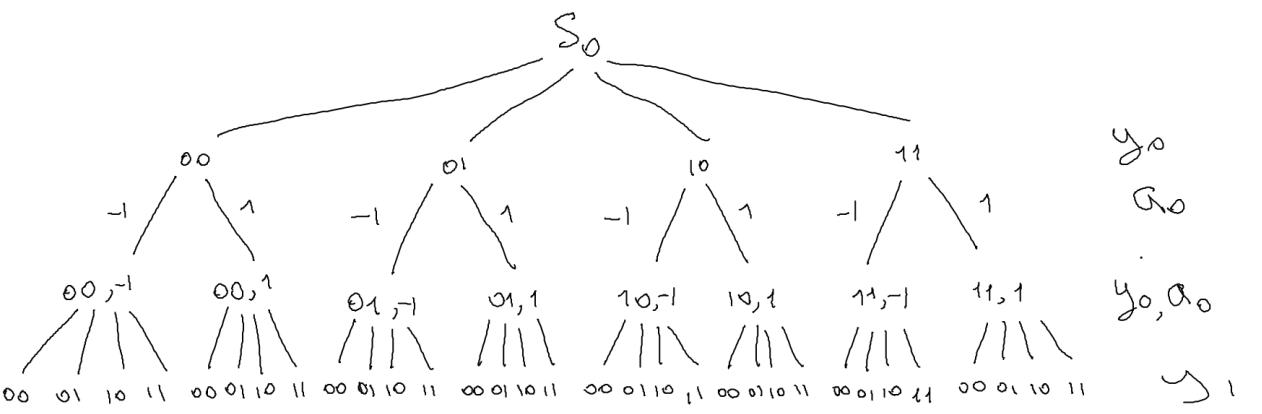
\includegraphics[width=0.5\textwidth]{../pics/ex31a.png}
\item For four nodes the state can be inferred: \\
for $[y_0 = 00, a_0 = -1, y_1 = 11]$ the only possible state is $s_1 = 0$ with $s_0 = 1$ \\
$[y_0 = 00, a_0 = 1, y_1 = 11]$ : $s_1 = 0$ $(s_0 = -1)$ \\
$[y_0 = 11, a_0 = -1, y_1 = 00]$ : $s_1 = -1$ $(s_0 = 0)$ \\
$[y_0 = 11, a_0 = 1, y_1 = 00]$ : $s_1 = 1$ $(s_0 = 0)$ \\
  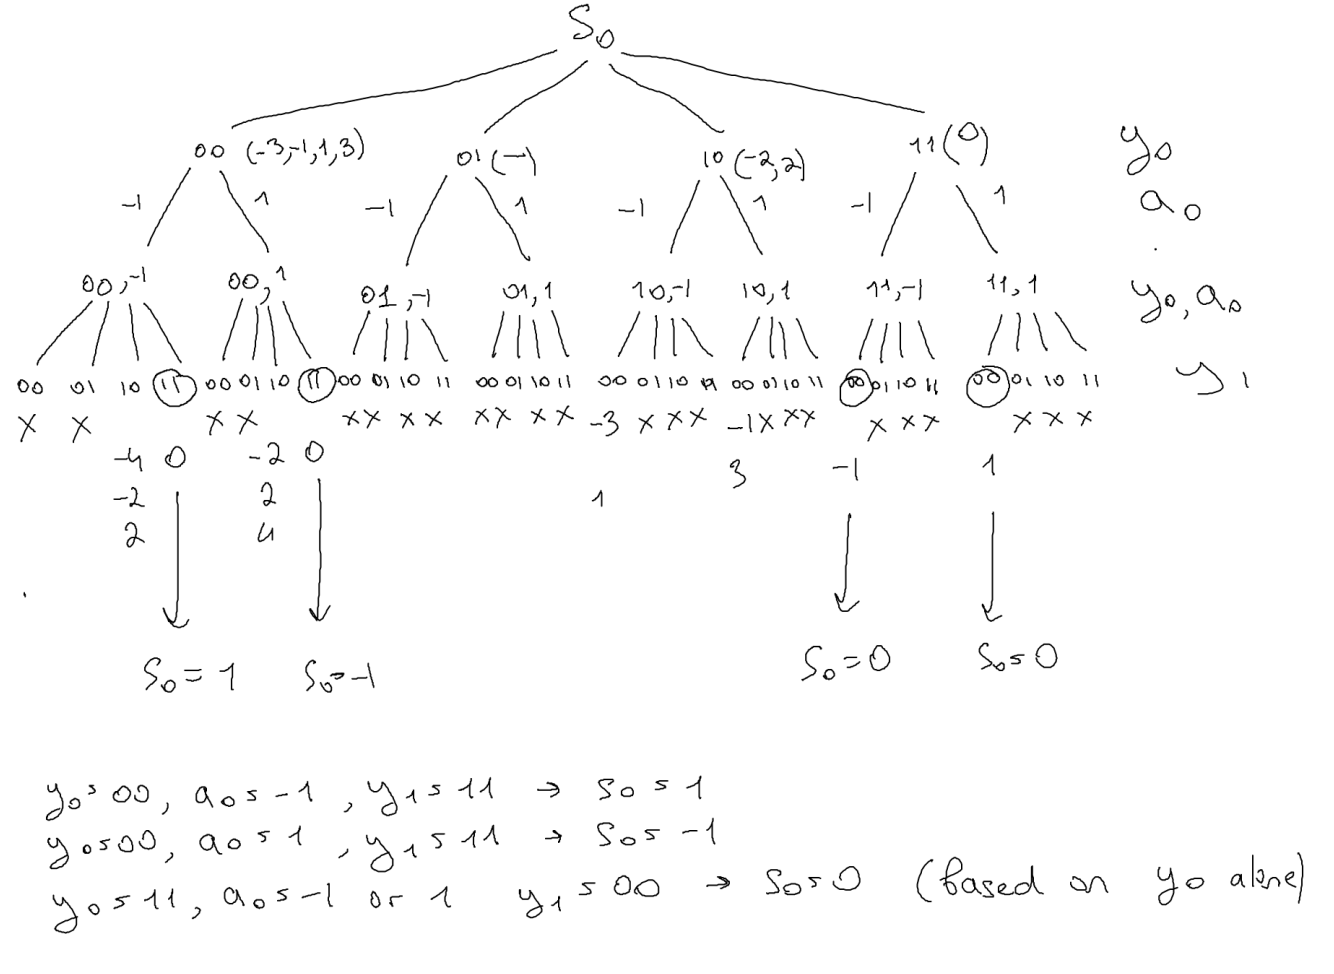
\includegraphics[width=0.5\textwidth]{../pics/ex31a2.png}
\item 24 of the 32 nodes can be pruned (marked with crosses).
\item for example the observation $y_0 = 00$ is possible for states $-3, -1, 1, 3$, the observation $y_0 = 01$ is not possible, etc (s. drawing)
\end{enumerate}


\end{solution}

%%%%%%%%%%%%%%%%%%%%%%%%%%%%%%%%%%%%%%%%%%%%%%%%%%%%%%%%%%%%%%%%%%%%%%%%%%%%%%%%

\exsection{Decision Tree for a Markov Decision Problem (1 Pt)}

Consider the following MDP:
\begin{itemize}
\item The state space is $s_t \in \ZZZ$, and the state is fullly observable.
\item The action space is $a_t \in\{-1, +1\}$
\item The state transition probabilities are
$$P(s'|s,a) = \begin{cases} .8
& \text{if~} s'=s+a \\ .2 & s'=s-a \\ 0
& \text{otherwise}\end{cases}$$
\item The initial state distribution is $P(s_0) = [s_0=0]$ (1 for $s_0=0$ and
zero otherwise)
\item The reward is binary with probability $P(r\=1|s) = [s=2]$
(reward of 1 for $s=2$ and zero otherwise)
\end{itemize}

\begin{enumerate}
\item Write (on paper) the decision tree for this domain, which has \emph{two} branchings: a 2-way branching for your decision $a_t\in\{-1,+1\}$, and a 2-way branching for the uncertain state transition.

Write down 4 levels of the tree, branching at $a_0,s_1,a_1,s_2$. (Warning: This has up to 16 leaf nodes.) You might want to ``compress'' the tree into a graph -- you're welcome to do this. BUT: what if decision $a=+1$ would add a negative reward (cost) of -1. Would it then still be ok to compress the tree into a graph?)

\item What is the expected return (=sum of rewards) of first deciding $a_0=+1$ and $a_1$ uniform random, versus $a_0=-1$ and $a_1$ uniform random? (Assuming the MDP stops after two transitions.)

\item What is the best expected return one can achieve, assuming the MDP stops after two transitions.
\end{enumerate}


\begin{solution}
\begin{enumerate}
\item the tree with 4 levels:
  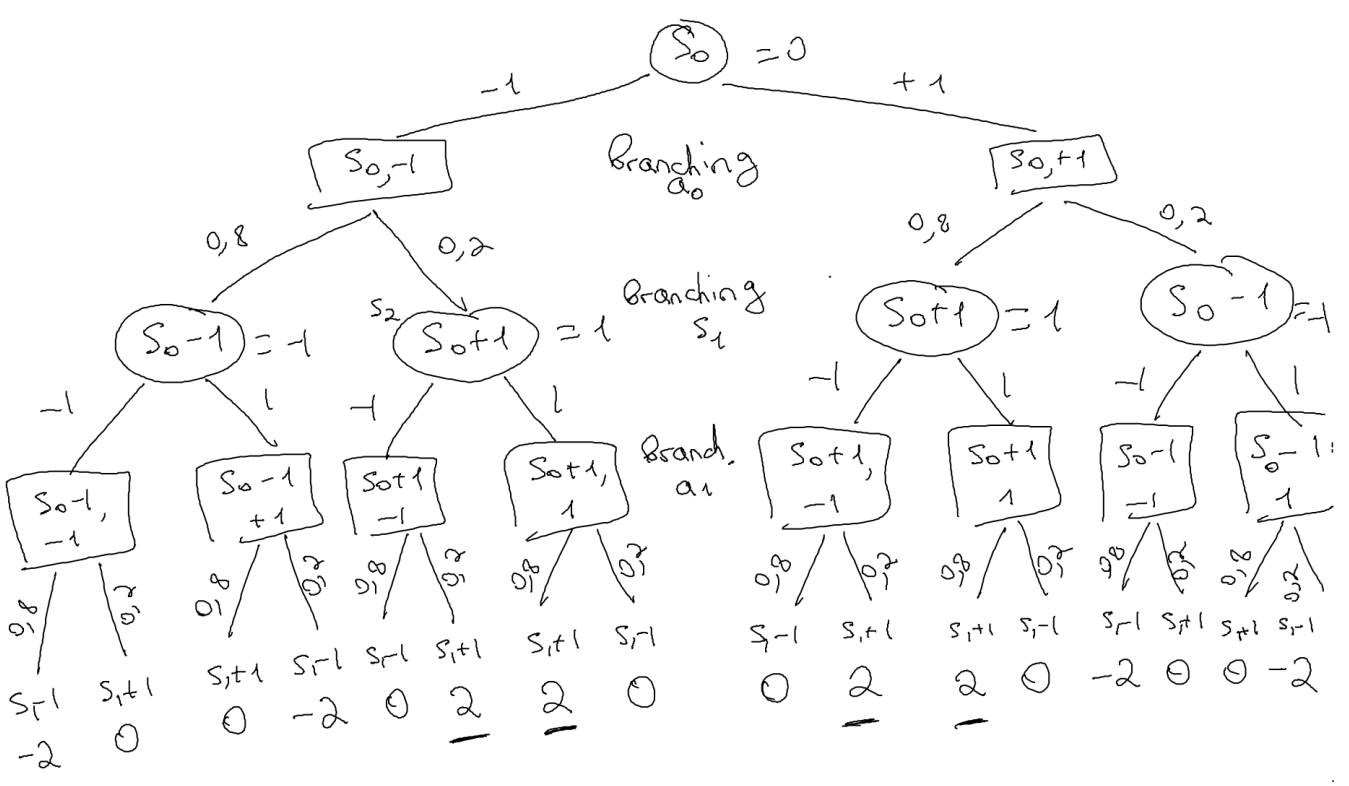
\includegraphics[width=0.5\textwidth]{../pics/ex32a.png}
\\
In the presence of a negative reward we cannot compress the tree, as every transition for decision $a=+1$ would change the accumulated reward. To calculate the reward we would need the full trajectory.


\item the expected reward for $a_0 = -1$ and $a_1$ uniform random is 0.1, with only two possible trajectories having non-zero reward \\
$E[r | a_0 = -1] = 0.2 * 0.5 * 0.2 * 1 + 0.2 * 0.5 * 0.8 * 1 + (..) * 0 = 0.1$\\
the expected reward for $a_0 = +1$ and $a_1$ uniform random is 0.4, again with only two possible trajectories having non-zero reward \\
$E[r | a_0 = +1] = 0.8 * 0.5 * 0.2 * 1 + 0.8 * 0.5 * 0.8 * 1 + (..) * 0  = 0.4$\\
\item for $a_0 = +1$ and $a_1 = +1$ the expected reward is 0.64 \\
$E[r | a_0 = +1, a_1 = +1] = 0.8 * (0.8 * 1 + 0.2 * 0) + 0.2 * 0 = 0.64$
\end{enumerate}


\end{solution}

%%%%%%%%%%%%%%%%%%%%%%%%%%%%%%%%%%%%%%%%%%%%%%%%%%%%%%%%%%%%%%%%%%%%%%%%%%%%%%%%

\exsection{Linear Regression and Bootstrapping by Hand (1 Pt)}

To be able to compute something by hand, we keep this very minimalistic here: Consider the data set $D=\{(-1,-1), (+1,+1)\}$ with just two data points $(x,y)$ with 1D input/output. Linear regression (with features $\phi(x) = (1,x)^\T$) would of course predict a linear function with slope 1 and offset 0, i.e., $f(x) = w_1 + x w_2$ with $w=(0,1)$.

\begin{enumerate}
\item Derive this solution from minimizing the loss $\sum_{i=1}^n (y_i - f(x_i))^2$ -- ideally using matrix notations to train you in this.
\item If you generate a randomized variant $\tilde D$ of the data using bootstrapping (resampling with replacement), what are the possible data sets $\tilde D$ that could be generated, and what are their probabilities?
\item What would be optimal linear regressor for each possible $\tilde D$?
\item Now, how would you estimate confidence bounds for the prediction at $x=0$ and $x=10$, based on bootstrapping?
\end{enumerate}

\begin{solution}
    \begin{enumerate}
        \item We define $Y = \[y_1, ..., y_n\]^T$, $\Phi = \left(\begin{array}{ccc}\phi_1(x_1) & .. & \phi_F(x_1) \\ & \vdots & \\ \phi_1(x_n) & .. & \phi_F(x_n)\end{array}\right)$, $W = (w_1, ..., w_F)^T$.
        In our case, as we have two features, we have $F = 2$, and $\phi_1(x) = 1, \phi_2(x) = x$.

    In matrix notation, we can write the loss function as $||Y - \Phi W||_2$.
    To find the optimum, we compute the derivative wrt. $W$, and set it to $0$. We use $W^*$ to denote the optimal linear regressor.
    Thus, 
    $
        2\Phi^T\Phi W^* - 2\Phi^TY = 0
    $
    and finally, $W^* = (\Phi^T\Phi)^{-1}\Phi^TY$
    \item The possible datasets are $\tilde D_1 = \{(-1, -1), (-1, -1)\}$, $\tilde D_2 = \{(1, 1), (1, 1)\}$, $\tilde D_3 = \{(-1, -1), (1, 1)\}$ with probabilities $\frac{1}{4}$, $\frac{1}{4}$, $\frac{1}{2}$, respectively.
    \item We can compute the optimal linear regressor by plugging in the values of the dataset into our formula from (a).
    For $\tilde D_3$, we obtain $w = (0, 1)$.

    When plugging in the values from datasets $\tilde D_1$ or $\tilde D_2$, the matrix $(\Phi^T\Phi)$ is not invertible, and the optimum linear regressor is not uniquely defined.

    Intuitively, this makes sense, as we only a have a single unique datapoint in these two datasets.
    \item With bootstrapping, we would evaluate the $x$ at each point to obtain the corresponding $y$ values. From all the predictions, we can then compute the mean, and standard deviation at these points.
    \end{enumerate}

\end{solution}


%%%%%%%%%%%%%%%%%%%%%%%%%%%%%%%%%%%%%%%%%%%%%%%%%%%%%%%%%%%%%%%%%%%%%%%%%%%%%%%%

\exerfoot

